%% ----------------------------------------------------------------
%% Thesis.tex -- MAIN FILE (the one that you compile with LaTeX) XD
%% ---------------------------------------------------------------- 

% Set up the document
\documentclass[a4paper, 11pt, oneside]{Thesis}

\usepackage[utf8]{inputenc}
\usepackage[nonumberlist, seeautonumberlist]{glossaries}
\newglossarystyle{mystyle}{%
  \glossarystyle{long}%
  \renewenvironment{theglossary}%
     {\begin{longtable}{p{3cm}p{\glsdescwidth}}}%
     {\end{longtable}}%
}
\usepackage[square, numbers, comma, sort&compress]{natbib}  % Use the "Natbib" style for the references in the Bibliography
\usepackage{hyperref}% http://ctan.org/pkg/hyperref

\usepackage{verbatim}  % Needed for the "comment" environment to make LaTeX comments
\usepackage{float}
\usepackage[refpage]{nomencl}
\usepackage{listings}
\usepackage{tabularx,ragged2e,booktabs,caption, makecell}
\usepackage{lipsum}
\usepackage{todonotes}
\usepackage[linesnumbered,algoruled,boxed,lined]{algorithm2e}
\usepackage{eurosym}      %<-- For EURO symbol 
\usepackage{filecontents}
\usepackage{enumitem}
\usepackage{placeins}
\usepackage{multirow}
\usepackage{array}
\usepackage{longtable}
\lstset{escapeinside={<@}{@>}}
\usepackage{subfig} 
\usepackage{float}
\usepackage{graphicx,subcaption}

\usepackage[toc,page]{appendix}



\makeatletter
\def\setChapterprefix#1{\gdef\@Prefix{#1}}
\setChapterprefix{}
\renewcommand*\l@chapter[2]{%
  \ifnum \c@tocdepth >\m@ne
    \addpenalty{-\@highpenalty}%
    \vskip 1.0em \@plus\p@
    \setlength\@tempdima{1.5em}%
    \begingroup
      \parindent \z@ \rightskip \@pnumwidth
      \parfillskip -\@pnumwidth
      \leavevmode \bfseries
      \advance\leftskip\@tempdima
      \hskip -\leftskip
      \@Prefix 
      #1\nobreak\hfil \nobreak\hb@xt@\@pnumwidth{\hss #2}\par
      \penalty\@highpenalty
    \endgroup
  \fi}
    \makeatother


\makeatletter
\renewcommand\fps@figure{!htb}
\setlength\@fptop{0pt} 
\makeatother
\renewcommand{\floatpagefraction}{.6}% before: .5 
\renewcommand{\textfraction}{.15} % before: .2 
\renewcommand{\topfraction}{.8}     % before: .7 
\renewcommand{\bottomfraction}{.5}  % before: .3 
\setcounter{topnumber}{3} % before: 2 
\setcounter{bottomnumber}{1} % before: 1 
\setcounter{totalnumber}{5} % before: 3 

\usepackage{url}

\usepackage{dirtytalk}
\usepackage{notoccite}
\usepackage{comment}
\usepackage{amsmath}
\usepackage{amssymb}
\usepackage{listings}
\usepackage{afterpage}
\usepackage{subfig}
\graphicspath{ {images/} }

\setlist{nolistsep}
\lstset{basicstyle=\ttfamily,
	showstringspaces=false,
	commentstyle=\color{red},
	keywordstyle=\color{blue}
}
\lstset{aboveskip=20pt,belowskip=20pt}


\newcommand\blankpage{%
	\null
	\thispagestyle{empty}%
	\addtocounter{page}{-1}%
	\newpage}

\SetKwProg{Fn}{Function}{}{}

% Make a glossary and a list of acronyms
\makeglossaries
% Glossary entries
\newglossaryentry{IT}{name={\textbf{IT}},%
    description={\textbf{I}nformation \textbf{T}echnology},%
}
\newglossaryentry{URI}{name={\textbf{URI}},%
    description={\textbf{U}niversal \textbf{R}esource \textbf{I}dentifier},%
}
\newglossaryentry{RDF}{name={\textbf{RDF}},%
    description={\textbf{R}esource \textbf{D}escription \textbf{F}ramework},%
}
\newglossaryentry{RDFS}{name={\textbf{RDFS}},%
    description={\textbf{R}esource \textbf{D}escription \textbf{F}ramework \textbf{S}chema},%
}
\newglossaryentry{OWL}{name={\textbf{OWL}},%
    description={\textbf{W}eb \textbf{O}ntology \textbf{L}anguage},%
}
\newglossaryentry{SWRL}{name={\textbf{SWRL}},%
    description={\textbf{S}emantic \textbf{W}eb \textbf{R}ule \textbf{L}anguage},%
}
\newglossaryentry{ACO}{name={\textbf{ACO}},%
    description={\textbf{A}ccess \textbf{C}ontrol \textbf{O}ntology},%
}
\newglossaryentry{ACC}{name={\textbf{ACC}},%
    description={\textbf{A}ccess \textbf{C}ontrol \textbf{C}omponent},%
}
\newglossaryentry{RDF-MTs}{name={\textbf{RDF-MTs}},%
    description={\textbf{R}esource \textbf{D}escription \textbf{F}ramework \textbf{M}olecule \textbf{T}emplates},%
}

\glsaddall

%------------------------------------------------------------------------------

%% ----------------------------------------------------------------

\begin{document}
\frontmatter      % Begin Roman style (i, ii, iii, iv...) page numbering
% Set up the Title Page
\title{RDF Doctor: Holistic RDF Syntax Validation and Error Correction}
\authors  {\texorpdfstring
            {{Ahmad Hemid}}
            {Ahmad Hemid}
            }
\addresses  {\groupname \deptname \univname}  % Do not change this here, instead these must be set in the "Thesis.cls" file, please look through it instead
\date       {\today}
\subject    {}
\keywords   {Access Control}
\maketitle
\blankpage
%% ----------------------------------------------------------------

\setstretch{1.3}  % It is better to have smaller font and larger line spacing than the other way round--

% Define the page headers using the FancyHdr package and set up for one-sided printing
  % Clears all page headers and footers
\rhead{\thepage}  % Sets the right side header to show the page number
  % Clears the left side page header

\pagestyle{fancy}  % Finally, use the "fancy" page style to implement the FancyHdr headers

%% ----------------------------------------------------------------
% Declaration Page required for the Thesis, your institution may give you a different text to place here
\Declaration{

% \addtocontents{toc}{\vspace{1em}}  % Add a gap in the Contents, for aesthetics


I, Ahmed Hemid, declare that this thesis, titled ``RDF Doctor: Holistic RDF Syntax Validation and Error Correction'', and the work presented in it are my own. I confirm that:

\begin{itemize} 
\item This work was done wholly or mainly while in candidature for a research degree at this University.
\item Where any part of this thesis has previously been submitted for a degree or any other qualification at this University or any other institution, this has been clearly stated.
\item Where I have consulted the published work of others, this is always clearly attributed.
\item Where I have quoted from the work of others, the source is always given. With the exception of such quotations, this thesis is entirely my own work.
\item I have acknowledged all main sources of help.
\end{itemize}

Ahmed Hemid
  
Signature:\\
\rule[1em]{25em}{0.5pt}  % This prints a line for the signature
 
Date:\\
\rule[1em]{25em}{0.5pt}  % This prints a line to write the date
}
\clearpage  % Declaration ended, now start a new page

%--------------------------------------------------------------

%% ----------------------------------------------------------------
% The "Quote Page"
%\pagestyle{empty}  % No headers or footers for the following pages
%
%\null\vfill
%
%\textit{``What we do in life ... echoes in eternity``}
%
%\begin{flushright}
%	`Gladiator` movie (2000)\\
%\end{flushright}

\vfill\vfill\vfill\vfill\vfill\vfill\null
\clearpage  %Quote page ended, start a new page
%% ----------------------------------------------------------------

\acknowledgements{
%	% \addtocontents{toc}{\vspace{1em}}  % Add a gap in the Contents, for aesthetics
	
%I would like to express my gratitude to every individual who assisted me with completing this scientific work, namely \textit{Prof. Dr. Maria-Esther Vidal} and \textit{Dr. Ioanna Lytra} for their continuous support and valuable directions.
I would like to say thank for 

\begin{itemize}
	\item My parents
	\item My wife 
	\item My children
\end{itemize}
 for their continuous support and long patience.

\hfill
Ahmed
}

% \clearpage  % End of the Acknowledgements
\afterpage{\blankpage}
%% ----------------------------------------------------------------

\pagestyle{fancy}  %The page style headers have been "empty" all this time, now use the "fancy" headers as defined before to bring them back

%% ----------------------------------------------------------------

\tableofcontents  % Write out the Table of Contents

%% ----------------------------------------------------------------
%\lhead{\emph{List of Figures}}  % Set the left side page header to "List of Figures"
\listoffigures  % Write out the List of Figures

%% ----------------------------------------------------------------
%\lhead{\emph{List of Tables}}  % Set the left side page header to "List of Tables"
\listoftables  % Write out the List of Tables

\printglossary[style=mystyle, title=Abbreviations]
%\printglossary[style=mystyle, title=Abbreviations, sort=standard]

%% ----------------------------------------------------------------
%\lhead{\emph{List of Listings}}  % Set the left side page header to "List of Listings"
%\lstlistoflistings  % Write out the List of Listings

%% ----------------------------------------------------------------
\mainmatter	  % Begin normal, numeric (1,2,3...) page numbering


% The Abstract Page
%\addtotoc{Abstract}  % Add the "Abstract" page entry to the Contents
\abstract{
	% \addtocontents{toc}{\vspace{1em}}  % Add a gap in the Contents, for aesthetics
%Information privacy in the digital space has become a serious concern as huge volumes of private data is being collected, processed, and stored on an ongoing basis. Nowadays, more research is being conducted on the matter of information privacy and that is because any possible exposure of this private information, e.g. medical or financial records, may lead to unwanted consequences. Therefore, it is of high importance to keep access to personal information under control.  Our study investigates a novel solution to support personal information privacy by enabling a level of access control in an open linked data environment. We propose a framework to enforce data access policies in federations of RDF datasets. The proposed framework is typically integrated with SPARQL query engines as an access control layer. Our contribution comprises the design of an RDFS/OWL access control ontology used to model the access authorizations, and the development of an access enforcement mechanism based on the RDFS inference capabilities. The framework provides RESTful APIs for the management and validation of access authorizations. We empirically evaluated our framework in terms of completeness and effectiveness using the BSBM benchmark and MULDER query engine. The evaluation results prove the applicability of our approach in imposing access control without causing information loss or adding a considerable overhead to the overall query execution time.
%
%\textit{\small{Keywords: Access Control, Authorization, Linked Data, RDFS, RDF Molecule}}
%}	
\clearpage  % Abstract ended, start a new page
 %% ----------------------------------------------------------------


%% ----------------------------------------------------------------

%\input{chapters/introduction}
%\section{Background} \label{Sec:Background}   
   
%\input{chapters/related-work}
%%\input{chapters/motivating-example}
%\input{chapters/datamodel_approach}
%\section{Implementation} \label{Sec:Implementation}   

%\input{chapters/experimental-study}
%\input{chapters/conclustion-and-future-work}
%\input{chapters/appendices}
\chapter{Introduction}
\label{ch:introduction}



\section{Introduction}

%\begin{itemize}
%
%    \item What is the subject of the study? Describe the
%        economic/econometric problem.
%
%    \item What is the purpose of the study (working hypothesis)?
%
%    \item What do we already know about the subject (literature
%        review)? Use citations: {\it \citet{Gallant:87} shows that...
%        Alternative Forms of the Wald test are considered
%        \citep{Breusch&Schmidt:88}.}
%
%    \item What is the innovation of the study?
%
%    \item Provide an overview of your results.
%
%
%    \item Outline of the paper:\\
%        {\it The paper is organized as follows. The next section describes %the
%        model under investigation. Section \ref{Sec:Literature Review} %reviews the up-to-date research works.
%        and Section \ref{Sec:Results} presents the results. Finally, %Section
%        \ref{Sec:Conc} concludes.}
%
%    \item The introduction should not be longer than 4 pages.
%
%\end{itemize}




\par The usage of Resource Description Framework \(RDF\) model is recently increasing in diverse fields in computer science, such as Big Data, Machine Learning, Data Science, Data Management, etc. The RDF data model helps computing machines in processing of "meta-data" which is data about data, especially those data about web resources. Moreover, such computing machines will be smarter to understand the data represented in different RDF serialization formats. 

Since the RDF model can facilitate  exchanging of data between software applications and it can be also serialized in multiple formats, such as Turtle\footnote{\href{https://www.w3.org/TR/turtle/}{Turtle}}, N-Triples\footnote{\href{https://www.w3.org/TR/n-triples/}{N-Triples}}, N3\footnote{\href{https://www.w3.org/TeamSubmission/n3/}{N3}}, JSON-LD	\footnote{\href{https://www.w3.org/2018/jsonld-cg-reports/json-ld/}{JSON-LD}}, RDF{/}XML\footnote{\href{https://www.w3.org/TR/rdf-syntax-grammar/}{RDF{/}XML}}, and RDF{/}JSON	\footnote{\href{https://dvcs.w3.org/hg/rdf/raw-file/default/rdf-json/index.html}{RDF{/}JSON}}, then its  quality and correctness needs to be proved before proceeding of any further processing. Most of available  parsers which check for syntax errors in RDF, fail to detect more than one error, especially those represented in Turtle or N-Triples serialization formats. Therefore, there is a need to have more powerful tools that help in listing all such errors or at least most of them.%todo needs to show most used formats  


The motivation of this study is mainly  encouraged by the  tremendous RDF data representation and usage of either Turtle and N-Triples serialization formats in different ontologies and in various sciences, as well as, by the desire to offer a smart solution, capable of listing all or most of syntax errors, particularly, in those two formats. Besides the aim of the study to afford a user-friendly syntax checker of RDF formats, this tool should empower with the ability of recovering some of these syntax errors, essentially, when the errors are common and predefined, such as missing a colon or a dot.  

%TODO need to speak about related work and the outline the result 

The following text in this chapter are divided in a couple of sections to express our motivation of the study, present the problem statement, presents the challenges, list our research contributions, and finally outline how this thesis is structured.  

\subsection{Motivation}

This study was motivated by several software use cases, have as a requirement for their operating, syntax checking of RDF data when it comes as an input. As a motivating example, one of the use cases is discussed in {Figure \ref{Fig:Motivation}}. It describes a collaboration system for processing an input RDF data and let's assume it is performing machine learning classification and analysis. Indeed, in this case, a valid input to the system is required. The input data is initially verified against syntax errors for further data processing, if an error or more are found, the system will stop processing the input data and return a report of errors to the user. The current existing tools (as will be discussed in Chapter \ref{ch:related}) which check the RDF syntax of the input,  only assert that the input is  syntax-error-free. When the input has an error or more, those tools stop  parsing, and further handling, additionally, they report that error to the user. 

Another essential point the abruption of parsing when the first syntax error is found will introduce much complications. Assuming, the input RDF data contains, for example, 10 syntax errors. Normally, what is happening when an error is found, the system will proceed with no further processing, instead it will report the existence of an error, with other information about the error, such an error message, row, and column numbers where the error is occurred. Subsequently, the reported error is commonly corrected by the user to be sent again for re-checking of the syntax. To make it more complex, suppose the user has 10 syntax errors in his RDF input, then, the previous process steps of an input checking, an pause of parsing, an error notifying, and an error correction by the user has to be repeated for 10 times.  Furthermore, when the number of syntax errors increases, the number of error processing and correction processes increases by the same value. Also, imagine what is the consumed time and the work overload to process an input RDF data contains hundreds or thousands of errors.  

	\begin{figure}[ht]
		\begin{center}
			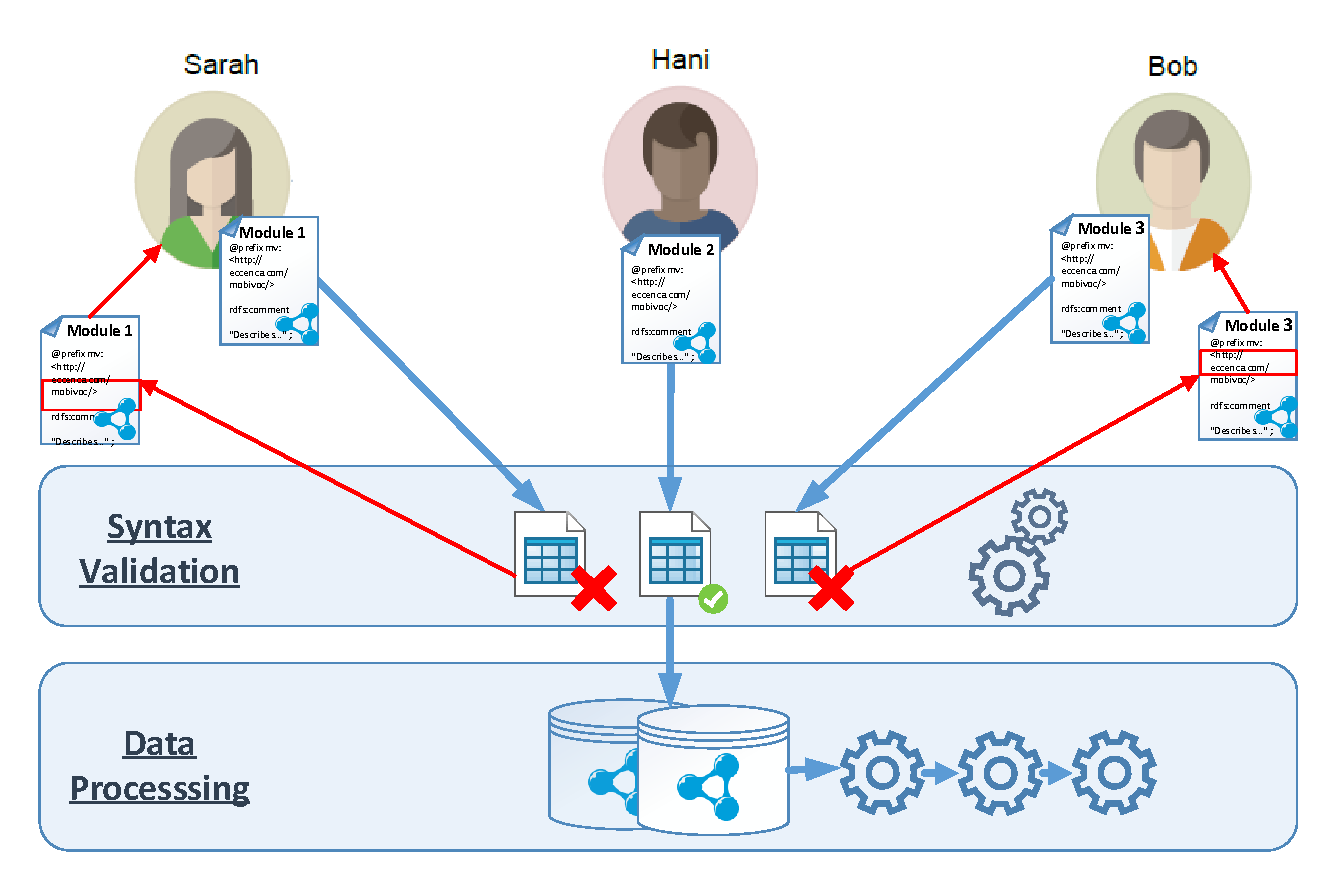
\includegraphics[scale=0.5,angle=0]{images/motivation}
			\caption{\textbf{A motivation example of syntax checking of data before further processing}}
			\label{Fig:Motivation}
		\end{center}
	\end{figure}

let's dig deep in demonstrating what is there in  {Figure \ref{Fig:Motivation}}, It is showing a flow of data from clients or users seeking further data processing. 3 persons are shown in this Figure, their names are Bob, Hani, and Sarah. All of them start with the first phase by sending their data to be syntactically checked. The parser starts checking if there are syntax errors of the input data, if such data passed with no syntax errors, it can be forwarded for further phases, i.e. for data processing, otherwise, the input data will send back to the user to correct the errors. {Figure \ref{Fig:Motivation}} clearly shows that Sarah and Bob have syntax errors in their input data,then, they got an error report, including details about the first detected error. In the meanwhile, Hani has received his data processed without getting such a report, since his input data has no syntax errors. 

This study has been fostered by the former illustrated example to find a suitable solution to allow the parser to continue the whole input of RDF data checking against syntax error and to list them in an error report if any was found. Therefore, the proposed solution focuses on producing a software tool that can detect all syntax errors that can be detected in the input RDF data. 

%\section{Objectives}
\section{Problem Description } 	
The research problem of this study is the unavailability of software tools that can list all the existing syntax errors in RDF files; thus, ontology engineers and users can fix them in one shot. Hence, such a list of errors if it is provided at the end of the syntax checking phase, it significantly assists to get rid of a loop of first error notifications, in case of an existence of multiple errors  in the input data as it was discussed.  

\section{Challenges }
Before reaching the proposed solution, different methods have been tired to reach the objective. The main purpose was the continuation of parsing till the end of the file without stopping on the first syntax error detection  and storing details of the detected errors into a data structure, such as lists. The following 3 tools were individually tested: Jena RIOT API\cite{McBride:2002:JSW:613357.613755}; RDF4J RIO API\cite{RDF4J:Online}; and  N3 Parser\cite{N3Parser:Online}. Both the first and the second are Java\_based RDF tool kit, including a plug-in for RDF parsing, the last is Javascript\_based parser, focused on N-Triple and Turtle serialization formats. In all of these framework, exception handling can be used to catch syntax errors. 

Our task was to remove the text that contains the first detected syntax error from an input text (since those tools fail when the first syntax error is found), then, to supply the remaining text for further parsing. Two methods were used: 1) cutting only the triple or the statement that contains the syntax error, 2) removing text before the found syntax error, including the statement of the error. Both those methods were failed to offer a suitable solution for continuation of parsing after an error discovery, for the following reasons: 1) the difficulty of handling nearby syntax errors, such as errors in the same line or in subsequent statements follow each others, 2) the inexpressive and incomprehensible of error messages, especially, in the second tool, which complicates understanding the actual syntax error for further handling.    


%TODO need references.


\section {Contributions}
In this study, the research work set out to syntactically check RDF data. 
The main contributions of RDF-Doctor (the name of output tool of this study) are:
\begin{enumerate}
	\item  {\bf Listing of detected syntax errors in RDF data:} it is a major goal and contribution where the intention to investigate RDF data, searching for syntax errors. RDF-Doctor is powered by ANTLR framework \cite{ANTLR:Website:Online}, a powerful parser generator, to establish an RDF parser that enables listing of all discovered syntax errors. To elaborate, the basis of the approach is the injection of error production rules inside the grammar which our parser is built based on. Once, the parser detects a combination of tokens from an RDF input that match one of these error production rules, it sends an error notification for an error listener where error lists are stored.
	\item {\bf Reporting syntax errors with user-friendly and expressive messages:} it is of great benefits for debugging and user\_based error corrections when a parser provides user-friendly and meaningful error messages to either normal users or ontology engineer. As the ancient Greek philosopher Socrates said, “Understanding a question is half an answer”\cite{Socrates:quote:Online}, likewise, an understandable error message helps to recover from an error.  RDF-Doctor is not only based on the regular expression input recognition, instead, its recognition is substantially based on grammar rules, each rule represents either a sequence of correct syntax tokens or a sequence of incorrect ones. In case of the latter, RDF-Doctor has a predefined information about each error, hence,  a customized error message can be formulated in an meaningful and convenient way and rendered on-the-fly to the error listener.  
	\item {\bf Automatic error recovery of some syntax errors:} commonly syntax errors in well-know programming languages are those types of missing a dot, adding more dots, or missing semicolon, similarly, happens in RDF data. To limit annoying conflicts while error correction, a certain rule has been set out to control the eligibility of an error to be corrected. The rule is the availability of this error in a predefined error correction list (it includes fundamentally common errors where the action of error recovery of an error is previously known to us), otherwise, it cannot be corrected. For example, on the one hand,  missing of a dot or a semicolon are common mistakes during editing of RDF data, those errors can proficiently correct by RDF-Doctor, but on the other hand, missing of a prefix declaration, decidedly, cannot be corrected since the details of that missing prefix are obscure and unknown.     
\end{enumerate}

\section {Thesis Structu
re}
The thesis is structured into 7 chapters. Until this spot, \textbf{Chapter \ref{ch:introduction}} was presented, titled with "Introduction". It  includes the general overview of the study, the motivation, the problem description and the challenges, research contributions are also introduced to show how our research work is differed from the state-of-art researches of other scientists. The
remainder of the thesis is organized as follows:
\begin{itemize}
	\item { \textbf{Chapter \ref{ch:preliminaries}:} presents the "Preliminaries" to shed light on the required background to understand what follows in the coming chapters.}
	
	\item {\textbf{Chapter \ref{ch:related}:}} reviews the "Related work" and presents the up-to-date research works. 
		
	\item {\textbf{Chapter \ref{ch:approach}:}} describes the "Approach" of the proposed solution. 
	
	\item {\textbf{Chapter \ref{ch:implementation}:}} demonstrates the "Implementation" of the proposed solution where its architecture and modules are exhibited.
	
	\item {\textbf{Chapter \ref{ch:evaluation}:}} shows the "Evaluation" part where the approach is tested and the results are discussed .

	\item {\textbf{Chapter \ref{ch:conclusions}:}} presents the "Conclusion" to complete this study.
\end{itemize}




%TODO 1- to change the figure in this chapter and improve the caption



\chapter{Preliminaries}
\label{ch:preliminaries}


\section{RDF Model}
The "Semantic Web" \cite{W3C:SemanticWebTerm:Online} term  has appeared during the transformation process of Web Development from "Web of documents" to "Web of data", similar to those data are found in databases. W3C defines it as "the Web of linked data" . {\it Figure \ref{Fig:semanticWebStack} describes the Semantic Web Stack, proposed by W3C. It can be seen, that it contains several technologies to enable users of creating their own data stores on web, building vocabularies, and enforcing processing rules on such data.   
\vspace{5mm} %5mm vertical space
\par
In order to make data more and machine-readable, and easier for interchange, RDF Model \cite{W3C:RDF-Primer:Online} has been proposed. RDF Model plays the role of data interchange in the layered Semantic Web Stack and leverages the high-level with low-level semantic web tools as it is shown in {\it Figure \ref{Fig:semanticWebStack}. 

	\begin{figure}[ht]
	\begin{center}
		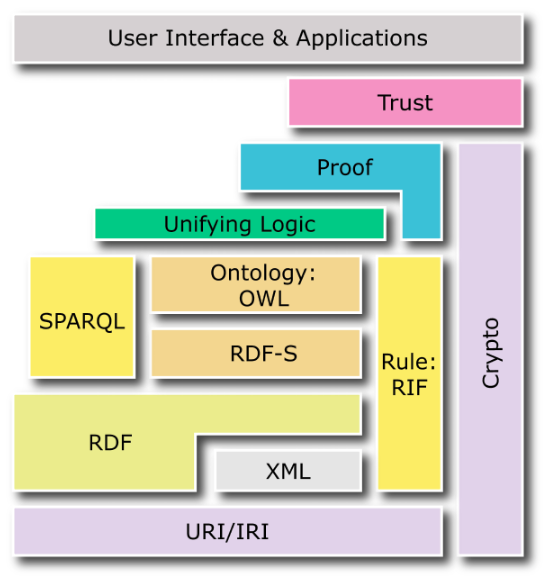
\includegraphics[scale=0.5,angle=0]{images/semanticWebStack}
		\caption{The Semantic Web Stack \cite{Bratt2007}}
		\label{Fig:semanticWebStack}
	\end{center}
\end{figure}
\vspace{12mm} %5mm vertical space
\par
{\it Figure \ref{Fig:rdfModel}(a) exhibits RDF Model's representation of data in triples. A triple is defined by 3 main players: subject, predicate, and object. It has a common similarity of a basic structure of simple sentence which consists of a subject, an object, and a verb. As the verb shows a relation or an event between the other two entities, similar, the predicate connects both subject and object in a certain relation. 
	
\begin{figure}[ht]
	\begin{center}
		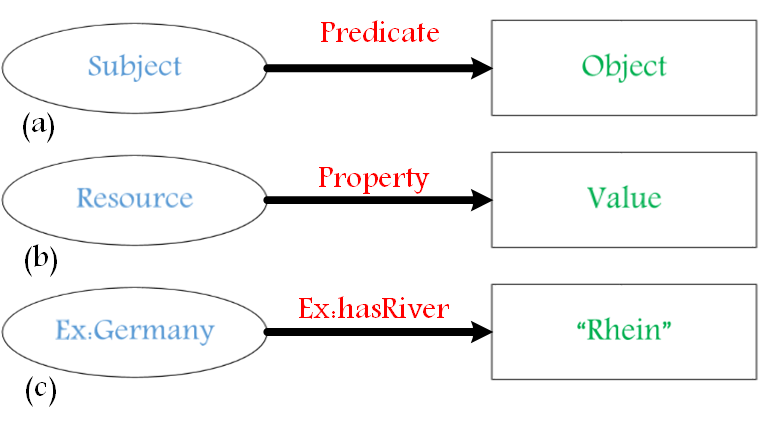
\includegraphics[scale=0.4,angle=0]{images/RDF-Model}
		\caption{RDF Model's Structure}
		\label{Fig:rdfModel}
	\end{center}
\end{figure}
 
A similar Resource-Property-Value structure to Subject-Predicate-Object of RDF Model's representation is drawn in {\it Figure \ref{Fig:rdfModel}(b). It is same representation but Subject, Predicate, and Object are replaced with Resource, Property, and Value in sequence.  
\subsection{Simple RDF Model Example}

To make it more clear, a simple example of RDF Modeling is giving in {\it Figure \ref{Fig:rdfModel}(c). To represent a fact that "German has The Rhein river", Ex:Germany is Subject/Resource, Ex:hasRiver is Predicate/Property, and "Rhein" is Object/Value. The first two value are Uniform Resource Identifiers (URIs) where "Ex:" is a defined path in RDF files and the following part is an extension of the path. The last value "Rhein" is a literal or a string. More examples can be viewed at \cite{W3C:RDF-Primer:Online}.

\section{Parsing and Error Recovery}
\subsection{Parsing and Grammar Definitions}
It is of great benefit to shed a little light on parsing topic to understand later the approach of this study. In \cite{parsingGuide2017}, Gabriele Tomassetti has defined \textbf{Parsing} by:

	\textbf{``The analysis of an input to organize the data according to the rule of a grammar''}. It can be intelligibly recognized that parsing deals with some input data and tries to analyses it based on a given grammer. let's have a look on the definition of grammer based on  \cite{parsingGuide2017}. \textbf{Grammer} is 
\textbf{``A formal grammar is a set of rules that describes syntactically a language''}. In the definition, rules are the significant part of the grammar to define the language's syntax.  
\subsection{Parser's Role}
The parser is an essential part in a compiler. {\it Figure \ref{Fig:parserPosition}} draws the role of the parser in a compiler. The first phase "Lexical Analyzer" receives the input data, then produces tokens for the next phase "Parser". Parser constructs a parse tree based on its grammar rules and gets the next token till it consumes all tokens. The parse tree as an parser's output is delivered to the next phases of a compiler. If any errors are found, lexical errors can be generated by Lexical Analyzer and Parser is the producer of both Syntax and semantic errors.%TODO{we can add more declartion about symbol table}
 A symbol table is data structure entries to store some declared values in the input, such as in programming languages object and variable names. It is used by both  Lexical Analyzer and Parser as it is shown in {\it Figure \ref{Fig:parserPosition}}.
%TODO{add the ref or change the image}

\begin{figure}[ht]
	\begin{center}
		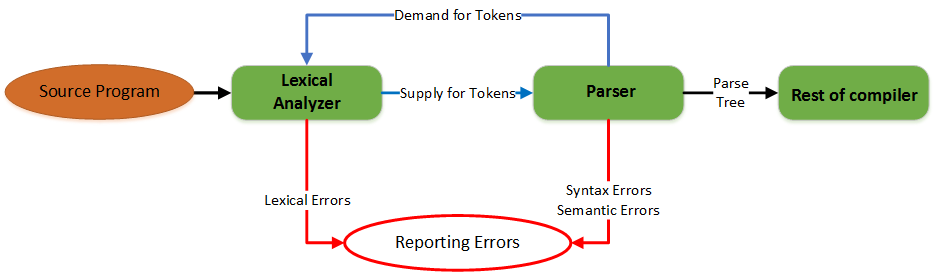
\includegraphics[scale=0.55,angle=0]{images/ParserRole}
		\caption{The Role of Parser}
		\label{Fig:parserPosition}
	\end{center}
\end{figure}
\subsection{Parser's Constructions}
In order to build a parser, there are two options to get such objective, either by building your own hand-written parser or getting an off-the-shelf parser generator tool. follows both approaches are discussed:
\par \textbf{1) Hand-writing Parsers:} someone writes his own parser, including the lexical analyzer and the parser. On the one hand this way gives more flexibility in handling several problems triggered during development but on the other hand it consumes much time and mind.
\par \textbf{2) Parser Generators:} someone uses a tool to generate a parser to do specific parsing task, by writing a compilable grammar to such tool. The most advantage of using those tools is the less consumed time to build a parser.  

\subsection{Error Recovery Methodologies in Parsers}
Error Recovery Strategies are the behavior of a system once an error is detected. Compiler's researchers Aho et al \cite{Aho2006}  have classified such methodologies as follows:
\begin{itemize}
	\item \textbf{Panic-Mode Recovery}: Once an error has been discovered, the parser ignores and skips next input symbols one by one till a recognized set of tokens is detected. In spite of discarding sometimes huge amount of input symbols with checking them for further error detection, it is considered a simple parsing mode and do not fall in an infinite loop while other modes may do.
	\item \textbf{Phrase-Level Recovery}: To continue the parsing process, the parser performs local correction. A typical local correction in RDF is to insert a missing dot or delete extraneous dots.
	\item \textbf{Error Productions}: By expecting the common errors, production rules can be inserted into the grammar. Then, the generated parser is well-informed about such errors. Error diagnostics can be easily done in this case since the error in our hand.
	\item \textbf{Global Correction}: The parser tries to reduce as much as possible number of change operations (Insertion, deletion or modification) when dealing with an incorrect input token to reduce globally total cost of error correction. To make it more clear, let's assume an incorrect input statement X is giving in grammar G, the parser constructs a closest error-free parse tree of statement Y to replace statment X, such that changes are small as possible. 
\end{itemize}


\section{ANTLR Parser Generator }
ANTLR is an handy tool and easy way to generate a specific domain language parser. It is an parser generator to do automatic generation of a source code of such parser without much coding and with less time. The basic principle used by ANTLR is define language's rules which draws the syntax and the semantic of the language the parser build for. 

\vspace{5mm} %5mm vertical space
\par
 As has been previously discussed, the compiler has two main subsystems: lexer and parser. Both lexer and parser are needed to have their rules defined in ANTLR grammar file.  {\it Figure \ref{Fig:ANTLR}} demonstrates an auto-generated parser program, generated based on ANTLR tool. follows is a sequence steps \citealp{ANTLR:Tool:Online}, describes such parsing process:

\begin{figure}[ht]
	\begin{center}
		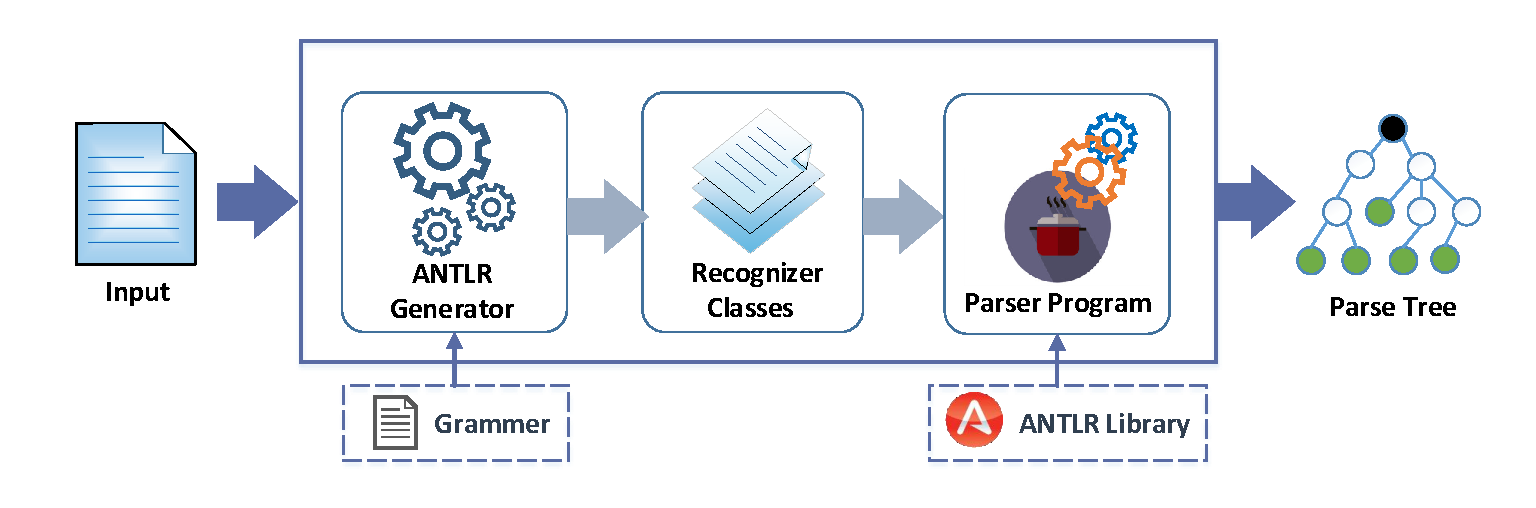
\includegraphics[scale=0.6]{images/ANTLR}
		\caption{Parsing process based on ANTLR parser generator}
		\label{Fig:ANTLR}
	\end{center}
\end{figure}


\begin{enumerate}
		
		\item  {\bf Writing a grammar file:} ordinarily, a grammar called a parsing expression grammar, or PEG is required to build a parser. ANTLR needs a context-free grammar, crafted with Extended Backus-Naur Form (EBNF). EBNF consists of a sequence of rules. These rules describe the syntax and the semantic of an input which needs to be parsed. Either Terminal or Non-terminal entities are the components of these rules. On the one hand, Terminals are the leaf elements where they have no grammatical structure, e.g., words or numbers. On the other hand, Terminal entities are those with a definite grammatical structure and name, e.g., triple component. 
		\item {\bf Generation of recognizer target\_based classes by ANTLR generator:} a significant feature of ANTLR is its capability of generated the auto-generated parse code for  a variety of the programming languages \citealp{ANTLR:Website:Online}: Java, C\#, Python (2 and 3), JavaScript, Go, C++, and Swift.
		\item {\bf Feeding an input file for parsing:} as an input, ANTLR can parse text documents without additional libraries. Users send their input files for parsing where the parsing process will be achieved based on the crafted grammar in the first step.
		\item {\bf Parsing procedure:} {\it figure \ref{Fig:ANTLR} } shows that it is the cooking time in this step where all materials and Ingredients are ready. The materials are: 1) the auto-generated parser, 2) the ANTLR library. The ingredients are one or more text files to be parsed. 
		\item {\bf Delivering of a report and parse tree as an output:} now the cake is ready for eating, an output of this process is given. A parse tree and a report of collected errors can be such output.
	\end{enumerate}












\chapter{Related Work}
\label{ch:related}


%In this chapter, we focus on previous work that is related to the problem stated in \nameref{ch:introduction}. 
In this chapter, we discuss the related work to our problem, i.e., research that has been realized in the field of RDF syntax parsing and checking.

\section{RDF Parsing and Syntax Checking}

There exist several tools for validating RDF data as an input.
Ontology engineers can either use tools that are available online or can download desktop applications for syntax validation.
These tools  can commonly detect only the first error while consecutively parsing input from its start point to its end. 
Therefore, semantic developers and engineers are struggling whilst debugging their RDF data, and they need alternative tools that could be more helpful. 
To the best of our knowledge, there is no fault-tolerant tool for parsing and syntax checking various RDF serializations which can detect multiple errors at the same time.  
Hence, a tool that can prominently list all errors included in the RDF data is of paramount importance.

\subsection{RDF/XML Parsing Tools}

Despite the existence of several theoretical models and practical tools that have been invented in the same field, we can hardly find  research that cares for finding more than one syntax error inside RDF data. 
During our journey of searching the existing tools that provide such a service, the W3C RDF validation tool \cite{W3C:Validation:Online} was firstly checked.
It is a web tool available online for the purpose of parsing and validating RDF/XML codes. 
It uses an Another RDF Parser (ARP) parser of Jena \cite{McBride:2002:JSW:613357.613755} as its core; However, it fails in detection of multiple syntax errors and shows only the first encountered error as it is shown in Figure \ref{Fig:errorW3RDFValidator}.
 
In 2000, a Validating RDF Parser (VRP) \cite{karsten:Thesis:2000} was developed by K. Tolle. In his thesis, 
VRP is a Java-based parsing tool with included features for semantically and syntactically checking dedicated for RDF/XML format. 
Nevertheless, the validation functionality provided by VRP is limited to parse only a format type of RDF/XML and does not support other RDF serializations, such as N3, N-Triple, or Turtle. 
Moreover, VRP is a desktop application tailored for human users, thus making it hardly usable from other applications while performing batch processing of several RDF documents at the same time.
Figure \ref{Fig:VRPErrorResult} shows that VRP can list more than one error or first detected error. 
An RDF/XML file with the same text applied in Figure \ref{Fig:errorW3RDFValidator}, included two syntax errors was used as an input to test VRP. 
As a result, four error messages were found. Two of them are related to the injected errors and significantly meaningful to correct them, whereas the other two messages are with no benefits and have no relation to the injected errors. 
In our work, a general approach that can work for all RDF serializations is envisioned; However, as use cases Turtle and N-Triple formats have been considered while developing RDF-Doctor to prove our assumption. 
 
 \begin{figure}[ht]
		\begin{center}
			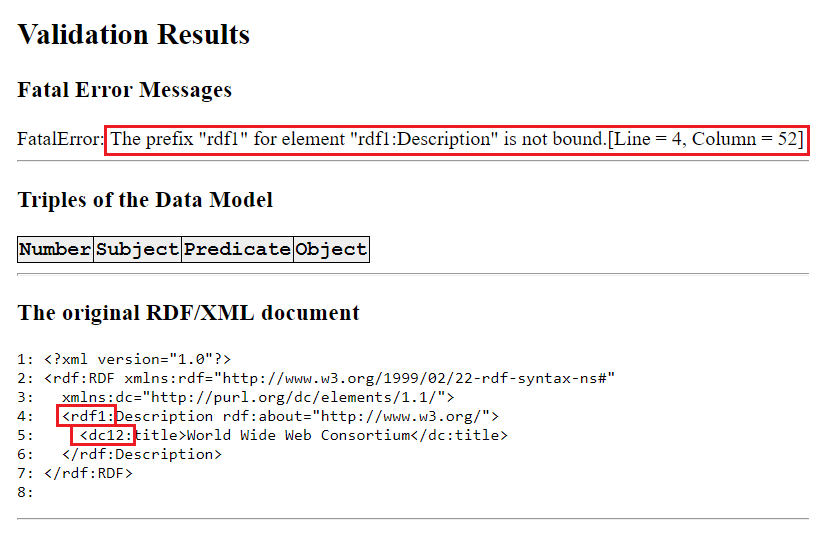
\includegraphics[scale=0.7,angle=0]{images/errorW3RDFValidator.png}
			\caption{\textbf{Validation results of the W3C RDF validation tool \cite{W3C:Validation:Online} after parsing an RDF/XML text, included two syntax errors.} The original RDF/XML document has two syntax errors since ``rdf1" and ``dc12" have no prefix declarations, but the results under ``Fatal Error Messages" show only the first found error and neglects the other.}
			\label{Fig:errorW3RDFValidator}
		\end{center}
	\end{figure}
\subsection{Several Serialization Formats Parsing Tools}

\par Next, the existing tools that validate more than one RDF serializations are checked. 
We have started with Jena RDF toolkit \cite{McBride:2002:JSW:613357.613755} which offers a validation service based on the ARP parser. 
It can be also used as a standalone program using a command-line or as an API integrated within another application.
Considering its powerful capability of validating numerous RDF serializations including RDF/XML, similarly, only the first encountered error is reported.

 \begin{figure}[ht]
		\begin{center}
			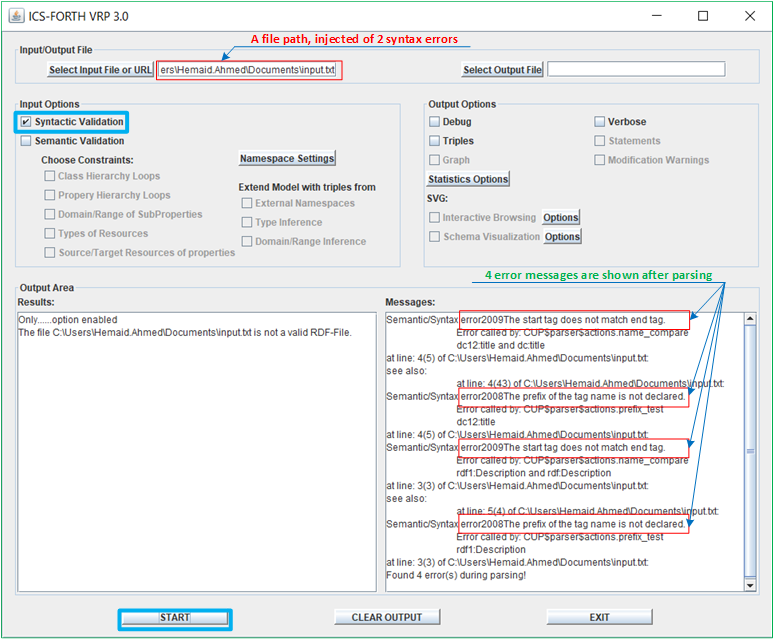
\includegraphics[scale=0.7,angle=0]{images/VRPErrorResult.png}
			\caption{\textbf{Results of Validating RDF Parser (VRP) \cite{karsten:Thesis:2000} after parsing an RDF/XML file.} Two errors are injected into the original RDF data. After the validation process, four error messages are shown, two of them are meaningful, whereas the other two messages have no meaning.}
			\label{Fig:VRPErrorResult}
		\end{center}
	\end{figure}
	
\vspace*{-\baselineskip}

\subsection{Classification of Parsing Approaches}

Approaches for validating various RDF serializations use the following core algorithms or methods as a significant part of their implementations. 
In the following, these core methods and their relations with concrete tools are discussed: 

\begin{itemize}[noitemsep] 

\item \textbf{ARP-parser-dependable approaches:} Both W3C RDF validation tool~\cite{W3C:Validation:Online} and RDF Validator and Converter~\cite{Mybluemix:Validation:Online} use the ARP parser of Jena framework \cite{McBride:2002:JSW:613357.613755}. 
The former validates only RDF/XML format whereas the later focuses more on triple-based serialization formats validating them and converting from one format to another. 

\item \textbf{N3-parser-dependable approaches:} This is mainly used by N3 parser~\cite{N3Parser:Online}, a JavaScript-based syntax validator, developed for checking the syntax of Turtle and N-Triple formats. 
The online version of IDLab Turtle Validator \cite{IDLab:Validation:Online} uses N3 parser and it is integrated as a NodeJS plug-in. 
The same approach was used to build a Turtle Editor with syntax validation in~\cite{petersenturtleeditor}. 
However, this approach is slow when parsing, and its behaviour is unpredictable when dealing with large files. 

\item \textbf{Shape expressions approaches:} In ~\cite{prud2014shape}, a Turtle parser was developed based on shape expressions \footnote{\url{https://www.w3.org/2001/sw/wiki/ShEx}}. 
Shape expressions describe the RDF graph based on regular expressions and validates RDF through declaring of constraints on the RDF data, if the declared constraints are violated, then RDF data is invalid, otherwise, it is valid. Furthermore, multiple tools we developed using the same approach in different programming languages, such as ShEx.js~\footnote{\url{https://github.com/shexSpec/shex.js}}, ShExJava~\footnote{\url{http://shexjava.lille.inria.fr/}}, Shaclex \footnote{\url{http://labra.weso.es/shaclex/}}, ShEx Ruby~\footnote{\url{https://ruby-rdf.github.io/shex/}}, PyShEx~\footnote {\url{https://github.com/hsolbrig/PyShEx}} built in JavaScript, Java, Scala, Ruby, Python, sequentially.

\item \textbf{Other parsing approaches:} Tools with another parsing method than the 3 listed above or unknown to us fall under this category. Raptor \footnote{\url{http://librdf.org/raptor/}} is a C-based open source library which includes parsers and serializers for a wide range of RDF serializations. 
It can be used as a standalone RDF parser. 
Also, Protege \footnote{\url{https://protege.stanford.edu/}}, is a free open source RDF editor, can work either as a desktop-based or a web-based application. 
It also supports several RDF serializations. Moreover, another variety of RDF parsers or tools: \cite{humfrey2010easyrdf},~\cite{RDF4J:Online},~\cite{krech2002rdflib} come
under  this category and the 2 last-mentioned parsers also failed to show more than the first syntax error.            
\end{itemize} 
\vspace*{-5mm}

The previous three approaches failed to list more than the first error at the same time. 
Moreover, an essential while processing a large number of RDF data is the performance, which is a weak point in the browser based tools such those implemented in JavaScript.

\section{Types of Error Messages}

Releasing user-friendly and meaningful error messages is of a great benefit to help the user to easily identify and correct the errors. 
\begin{itemize}
    \item \textbf{Non-expressive and meaningless error messages:} The parsing tools under the shape expressions approach like~\cite{prud2014shape} show less expressive and unfriendly error messages.
    \item \textbf{Expressive error and meaningful messages:} The parsing tools which utilize a ARP-parser-dependable approach like~\cite{N3Parser:Online},~\cite{Mybluemix:Validation:Online},~\cite{McBride:2002:JSW:613357.613755} or a N3-parser-dependable approach like~\cite{N3Parser:Online},~\cite{IDLab:Validation:Online},~\cite{petersenturtleeditor} are presenting more expressive and user-friendly error messages including its location in a proper way. 
    
\end{itemize}

\section{Error Recovery Approaches}
The existence of the automatic error recovery or correction feature is valuable to resolve from common syntax errors in RDF data.  Our survey of research papers and tools in relation to an auto-correction of RDF syntax errors shows that such a feature is not exit either theoretically or practically. %For example, a number of programming languages need a semicolon at the end of the line. 
%There are also few tools which can correct, such errors without the involvement of the programmer. 
%In the same way it will be useful to have this option of automatic correction after parsing of various serialization formats of RDF. 
However, Halilaj et al in \cite{Git4Voc:article} pointed out the need for this feature and explored its benefits.
Further, while searching other tools and approaches which have the same feature in other fields, \cite{AutoCorrection:Fix-it} was found.  \cite{AutoCorrection:Fix-it} reports about a Review Bot tool that can automatically review a source code using static analysis output and correct encountered syntax errors using the parser tree. Their approach is applicable in our case, but since a subset of common syntax errors are statically corrected in the current version of RDF-Doctor based on the collected error messages.    

\section{Summary}

Although there exist a number of tools developed over the years to deal with validation of RDF data from syntactic perspective, the majority of them fail in the first encountered error.
Moreover, several tools are limited only to the human users and do not provide any command-line or API interface.
Therefore, we foresee the need for a comprehensive approach able to identify all syntax errors at the same time and provide meaningful messages to help users to correct them.
In addition, a feature to automatically correct a number of common syntax errors is crucial to reduce time consumed for correction process.  

%after describing the actual issue, reviewing the state-of-art of research works, related to the same spot with pointing out the different approaches of RDF parsing and syntax checking, different types of error messages, and finally the approach of automatic error correction. 
%The outcome of this study is the RDF-Doctor. It is a parser that is generated with the help of the ANTLR parser generator. 
%Additionally, It is a Java\_based application to parse N-Triple and Turtle serialization formats; show a meaningful error messages; as well as, automatically recover from common syntax errors.    











\chapter{Approach}
\label{ch:approach}
%As has been discussed in Chapter \ref{ch:related}, there is a need for a tool which can detect all the encountered syntax errors in RDF documents to ensure their quality and to make RDF diagnostics easy for users instead of showing only the first detected syntax error, struggling them in finding the other syntax errors if exist. 
In this chapter, we present RDF-Doctor, an approach towards realization of a comprehensive parser for syntax validation and recovery.
RDF-Doctor is able to identify more than one syntax error at the same time and provide meaningful messages.
%order to fill this need, this study was held to propose a proper solution. 
Then, main components of RDF-Doctor are discussed in detail along with possibilities of integration serialization formats, such as Turtle and N-Triple. Finally, this chapter ends with presenting the categories of syntax errors.


\section{Overview of RDF-Doctor Approach}

This section covers the core component of the approach, then discusses the main processing steps, and ends with elaborating the categories of RDF syntax errors to ease the road to the appropriate solution. 

\subsection{ANTLR: The Core Component}

The core component inside RDF-Doctor is the ANTLR framework. It is used to automatically generate a parser based our developed grammar, including predefined error production rules to match sequences of tokens that contains RDF syntax errors.
%In order to find a parser which can accept the error production rules in its grammar, our choice was to use ANTLR framework to automatically generate the required parser.
%Equally important lots of handy features in ANTLR motivate its usage in the proposed solution to generate the internal parser, and also as an imported library for compiling and  running  of RDF-Doctor. 
The ANTLR framework has several important features: 1) a given grammar can equip with error production rules and when a couple of tokens match such rules, the parser will fire an error notification; 2) it uses a parse tree to parse input tokens and the view of this parse tree can be delivered as one of the outputs to the user at the end of parsing process; and 3)it supports the auto-generation of parsers in different programming languages.
%which is an one-to-many added value, where one grammar file can automatically generate of the programming languages.

%\begin{itemize}
% \item \textbf {Input}: It is the role of the user to provide an RDF file with certain options, such as 1) enabling/disabling of the error correction; 2) showing an error report of JSON\footnote{https://www.json.org/} or text format; and 3) concealing/showing up the parse tree.


%\item \textbf{Processing}: starts with preparing the input to be parsed in the following workflow: 1)it reads the input; 2) splits it into smaller pieces if needed; 3) parses the input for each slice (if many); and 4) corrects a subset of detected syntax errors. 
%This phase utilizes the parser built based on a predefined grammar.
%it requires ANTLR library for parsing, and some options from the user to activate/deactive some features of the solution.   
%\item \textbf{Output}: provides the reports after processing phase, %including 1) an error report to announce the detected syntax errors; 2) a correction report which lists the recovered syntax errors; and 3) an output file after healing some of the detected syntax errors\todo{It is not clear what is the point number 3}; and 4) a frame contains the parse tree. 
%Both, the correction report and the output file require to be enabled in order to be generated. 
%\end{itemize}


\subsection{Main Processing Steps}

\begin{figure}
	\centering
	  	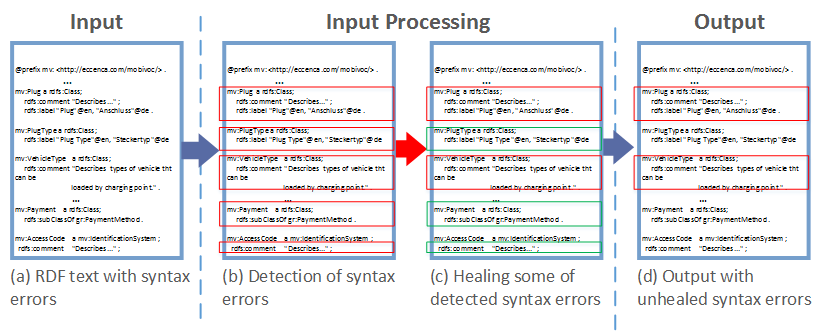
\includegraphics[width=1\textwidth]{images/Approach.png}
		\caption{\textbf{RDF-Doctor workflow.} The user writes or edits his own RDF file, then sends it to RDF-Doctor for parsing.
		Next, RDF-Doctor can divide the input in multiple chucks, in the case of a large input, or use the same input file. 
		Each input chunk or file is parsed to detect any syntax errors if they exist, then it recovers a subset of detected errors, if the automatic error recovery feature is enabled by the user. 
		Finally, RDF-Doctor outputs a parse tree, a correction report, an error report, and an output file, including an RDF file after error recovery.}
		\label{Fig:Approach}  
\end{figure}

The workflow of RDF-Doctor illustrated in Figure \ref{Fig:Approach} and its architecture depicted in Figure \ref{Fig:Architecture} are discussed in the significant steps of RDF-Doctor in the following:
%shows the technique used to handle an RDF text, including a couple of  syntax errors. 
%In the following, the main milestones of this approach are explained in 4 sequential steps:

 \begin{enumerate}[label=(\alph*)]
\item \textbf{Reading RDF files}: An ordinary RDF file is submitted to RDF-Doctor, this is the Input phase, as described in Figure~\ref{Fig:Approach} (a).
Initially, Processing components in Figure \ref{Fig:Architecture} read the submitted file. In the case that the file is too large (more than 1 million triples), then it is segmented into two or more chunks based on the number of triples. 
Each chunk is parsed and processed separately from others in this step.
%%%%%%%%%%%%%%%%%%%%
Moreover, certain options can be selected by the user before submitting the file, such as 1) enabling/disabling of the automatic error correction; 2) showing an error report in either  JSON~\footnote{\url{https://www.json.org/}} or text format; and 3) concealing/showing up the parse tree diagram at the end of parsing process.
%%%%%%%%%%%%%%%%%%%%
%{Figure \ref{Fig:Approach}}(a) simulates the actual work of this step where a submission of an RDF file with syntax errors is assumed. 
\item \textbf{Detecting of syntax errors}: Parsing is the third step in  the Process phase in Figure \ref{Fig:Architecture}, in which the parser has predefined rules for syntax errors,  %(these rules are titled with error production rules, presented in Error Recovery Methodologies in Chapter \ref{ch:preliminaries}), 
\begin{figure}[ht]
	\begin{center}
		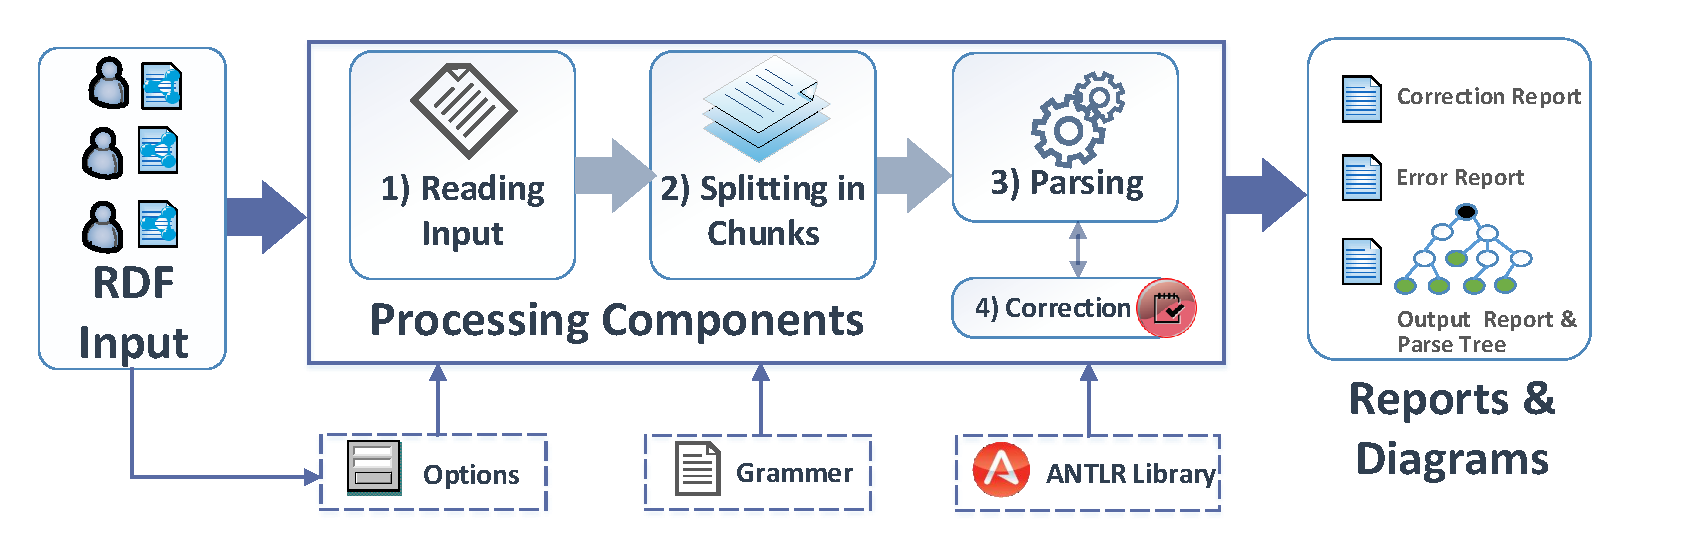
\includegraphics[scale=0.5]{images/architecture.pdf}
	\caption{\textbf{RDF-Doctor architecture.} It consists of Input, Processing, and Output phases. 
		In the Input phase, users send their RDF data. The Processing phase reads the data, splits them into smaller chunks if they are large, then continues parsing and recovery of certain errors.
		In this phase, a user action is required to enable/disable the error recovery.
	    Finally, the Output phase presents reports for error detection and recovered error, as well as a parse tree.}
		\label{Fig:Architecture}
	\end{center}
\end{figure}
once a rule is matched with a sequence of input tokens, it raises a flag to the error listener API which later is listed in the final error report. 
Reading of input tokens continues until the end of the file while searching for any match in order to identify potential syntax errors. 
In {Figure \ref{Fig:Approach}}(b) lines surrounded with \emph{red color} depict the detected lines which contain syntax errors.
%%%%%%%%%%%%%%%%%%%%%%%
%%%%%%%%%%%%%%%%%%%%%%%
To have a deep thought on the internal works of the parser to detect syntax errors using a parse tree. Figure \ref{Fig:approachParseTree} shows how each sub-tree of the root node (acts as the starting rule) is a rule containing either a correct syntax or an incorrect one. Each rule is represented by a sub-tree being empty or one and more non-terminals (considered as rules in the grammar) and one and more terminals (they are lexical forms of input tokens). A sub-tree produces an syntax error, if all of its terminals (shown in \emph{red color} in Figure \ref{Fig:approachParseTree}) formulate an error production rule of grammar rules. Hence in both sub-trees 2\textsuperscript{nd} and 4\textsuperscript{th} from left-to-right over Figure \ref{Fig:approachParseTree} are rules with a sequence of tokens producing syntax errors.  Meanwhile other sub-tree 1\textsuperscript{st},  3\textsuperscript{rd}, and 5\textsuperscript{th} with terminals in \emph{green color}  are including  correct syntactic  forms.


\item \textbf {Healing a subset of encountered syntax errors}:%%%%%%%%%%%%%%%%%%%%
 { Figure} \ref{Fig:Architecture} shows this feature as the  4\textsuperscript{th} of processing components. %%%%%%%%%%%%%%%%%%%%
Firstly, it needs to be manually activated by the user, since it is disabled by default. Secondly, the method of syntax error recovery currently focuses on a certain type of errors which has only one predefined solution to correct them. Examples of such errors are  missing  a dot at the end of a triple, missing a semi-colon after multiple predicates sharing same subject, or missing a comma after multiple objects having same subject and predicate. Lines surrounded with \emph{green color} in {Figure~\ref{Fig:Approach}}(c) represent some of the healed lines from error at the end of the correction phase. 

\item\textbf {Producing of the output}: The output phase, demonstrated in Figure \ref{Fig:Architecture}, assumed the activation of automatic correction feature by the user. Additionally, {Figure \ref{Fig:Approach}}(d) describes how the output file looks like at the end of this phase.    It shows lines containing errors are already recovered, whereas other lines still are unhealed. Commonly, errors that cannot be recovered by RDF-Doctor without user intervention, are those errors which can have several solutions, for example, a literal with multiple language tags like ``me"@en@de which shows a string with two language tags and since the solution would be an omission of one of them but the intention of the user is unknown in this sense. In addition, there exist errors with undefined or unknown recovery solution, for example, missing of a user-defined prefix declaration for a certain local namespace which cannot be guessed since it is only known by the user himself. 
\end{enumerate} 
\begin{figure}
	\centering
	  	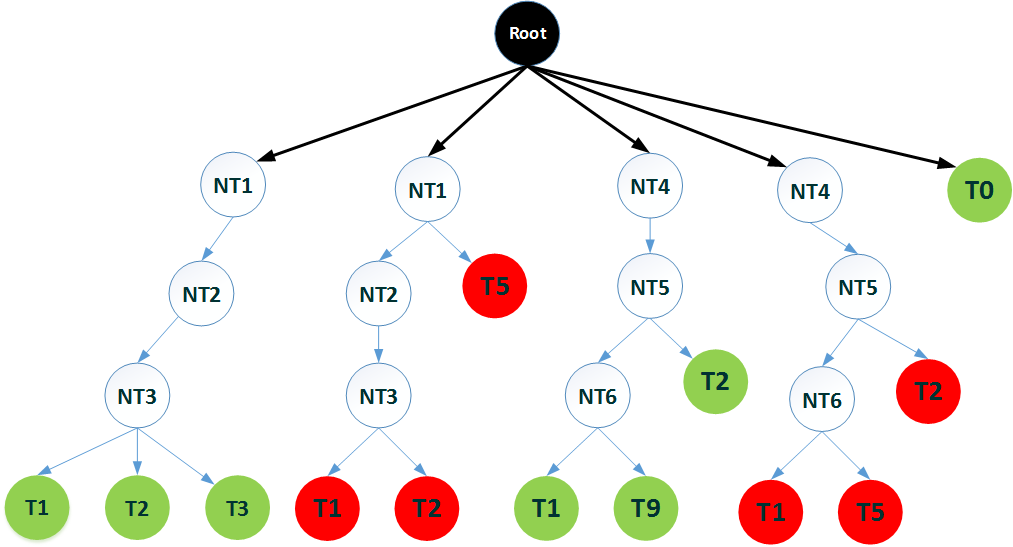
\includegraphics[width=.8\textwidth]{images/approachParseTree.png}
		\caption{\textbf{Detection of syntax errors while traversing the parse tree.} 
		Root node is the head of the first rule in the grammar and the head of the parse tree.
		All the children of the root are either non-terminal nodes represented by ``NT" followed by an number or  terminal ones shown by ``T" succeeded by a number. 
		A syntax error can be detected on a non-terminal node when all of its terminals represent a sequence of tokens that is a statement including a syntax error. Red terminals represent error-inclusive statements and green ones represent error-free statements.}
		\label{Fig:approachParseTree}  
\end{figure}


To functionally represent the approach of this study, Algorithm \ref{alg:algorithm-main} was engineered. 
It shows the abstract behaviour of RDF-Doctor where \textbf{syntaxRules} variable combines both correct syntax rules and incorrect ones. 
A \textbf{while loop} carries on until reaching the current end of file or chunk, if a large file is separated into several chunks. 
The \textbf{ruleToBeMatched} variable incloses one rule of either correct or incorrect production rules, formed by the supplied tokens. While the variable \textbf{currentTokens} stores a sequence of current supplied tokens to check to which rule, it belongs.  

Since the crucial step is to find encountered syntax errors, \textbf{ruleToBeMatched} is evaluated to check if its content is matched any of \textbf{incorrectSyntaxRules}. If this the case, then the content of \textbf{currentTokens} is considered as a syntax error, and the parser sends an error notification to any subscribed error listener API, in order to further process of the collected errors. 

\begin{algorithm}[] 
 \caption{The pseudo-code of RDF-Doctor}
 \label{alg:algorithm-main}
 \KwData{inputText, correctSyntaxRules, incorrectSyntaxRules, CorrectionIsSelected}
 \KwResult{foundSyntaxErrors and recoveredSyntaxErrors}
% S = subject(M)\;
foundSyntaxErrors = [ ];\\
recoveredSyntaxErrors = [ ];\\
$syntaxRules \leftarrow correctSyntaxRules + incorrectSyntaxRules;$\\
		\While{token in inputText \&\& $inputText \neq EOF$}{
		currentTokens += token;\\
ruleToBeMatched += lex(token);\\
		\uIf{ syntaxRules contains ruleToBeMatched}{
		\uIf{ incorrectSyntaxRules contains ruleToBeMatched}{
		 foundSyntaxErrors.push(currentTokens);\\
		\uIf{ CorrectionIsSelected}{
		\uIf{ canErrorRecovered(ruleToBeMatched)}{
		  \uIf{recoverSyntaxError(currentTokens)}{
		  recoveredSyntaxErrors.push(currentTokens);\\
		  foundSyntaxErrors.pop(currentTokens);\\

		  }
		}
		}
		}
		 $currentTokens \leftarrow ""$  \\
		 $ruleToBeMatched \leftarrow ""$  \\
		 $token \leftarrow ""$  	\\	
		}
}
return foundSyntaxErrors , recoveredSyntaxErrors
\end{algorithm}

The automatic correction of errors is a feature that can be activated as an additional option when running RDF-Doctor. 
In the case that the user selects to enable it, then the \emph{Error Correction Module} will traverse the entire list of detected syntax errors and based on the error message, it can identify if the error can be unquestionably corrected or needs a user intervention. 
At the end of the correction phase, a report of the corrected errors will be delivered to the user. 

\section{Categories of RDF Syntax Errors}

In this approach, Turtle and N-Triples RDF serializations are used as the use case syntaxes. 
Hence, Turtle is a special case of N-Triples. For this reason, the grammar of RDF-Doctor was created based on Turtle serialization. 
Furthermore, since the significant part in this study is the ability to identify syntax errors, the expected syntax errors need to be known in advance in order to be injected in the grammar. 
A suite of Turtle syntax errors are presented in ~\cite{TurtleTests:Online} plays an important role in syntax errors declaration. It contains several files in Turtle with an objective of showing both correct and incorrect syntaxes. Additionally, a filename in~\cite{TurtleTests:Online}, i.e., if it contains the word ``Bad", it means that it contains an incorrect syntax, which can be syntactically engineered in our grammar.

 \begin{table*}[tbp]
 	\centering
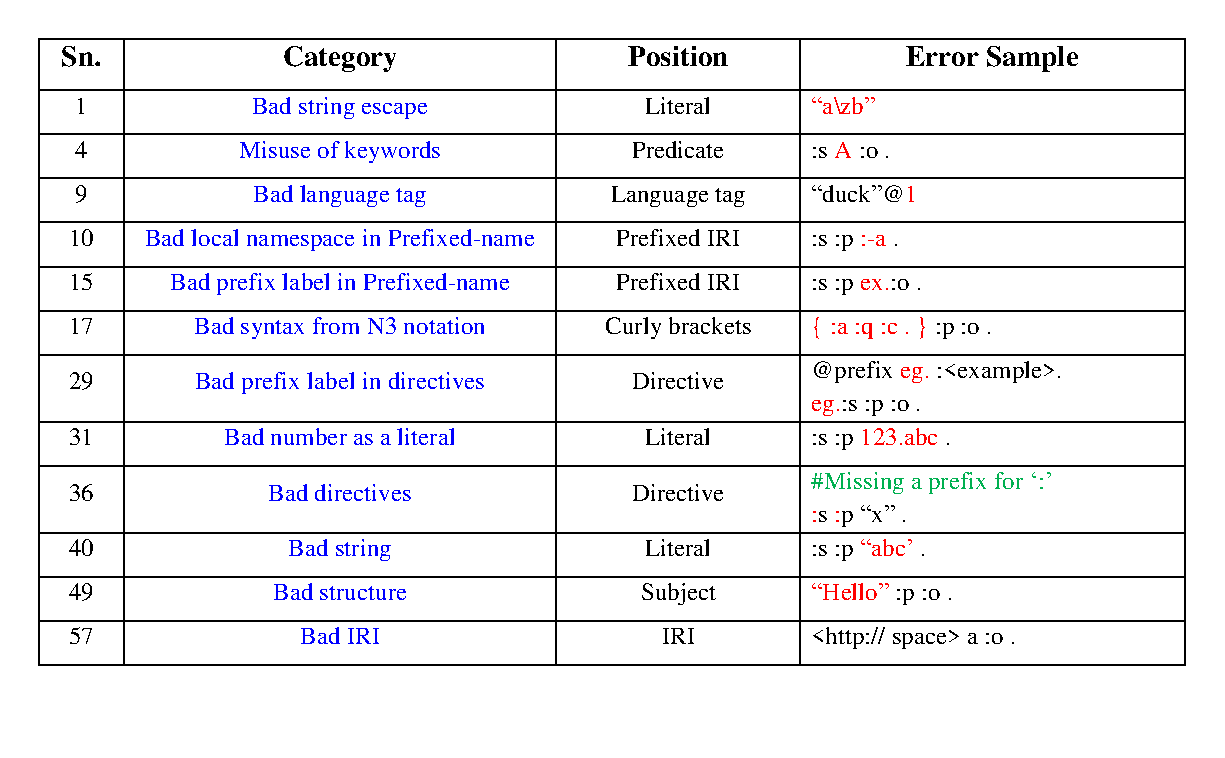
\includegraphics[width=5.5in]{images/TrimmedBigTable.pdf}
		\setlength\abovecaptionskip{-10mm}
	\caption{\textbf{Categories of a subset of syntax errors of N-Triple and Turtle serializations}.
	This table is a part of Appendix~\ref{tab:syntaxErrorCate} which shows one sample of each category. The serial numbers take the same order of rows in the referred table. 
	Position represents a term related to Turtle and N-Triple serializations where the actual syntax error is located.}
	\label{tab:trimmedTable}
\end{table*}


In table \ref{tab:trimmedTable}, we have categorized types of syntax errors into multiple categories. These categories are taking from the filenames in~\cite{TurtleTests:Online} with some modification to become meaningful. The table shows each category with one error sample and an error position where the actual syntax error is located. Indeed, this helps much in designing of the grammar rules and also to identify which of them can be automatically corrected. Details including more samples of these categories are provided in Appendix~\ref{tab:syntaxErrorCate}.     

\chapter{Implementation}
\label{ch:implementation}


In this chapter, details of the implementation practical part of the study is discussed. The architecture, modules, development tools, installation, and configurations of such part are the main role of this chapter.  
 
\section {Architecture}
The design of the architecture was planned based on the Input-Process-Output Model. It can be also considered as a black-box solution where the solution processes the input, then it delivers the output once it is ready. follows is the discussion of those 3 phases, described in Figure \ref{Fig:Architecture} : 
 \begin{figure}[ht]
	\begin{center}
		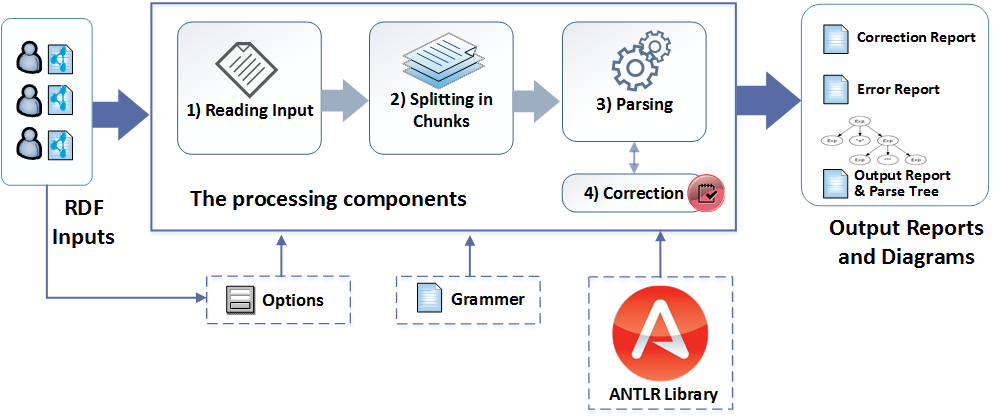
\includegraphics[scale=0.5,angle=0]{images/Architecture}
		\caption{The proposed solution architecture}
		\label{Fig:Architecture}
	\end{center}
\end{figure}
 \begin{itemize}
 \item \textbf {Input}: It is the role of the user to supply an RDF text with certain options, such as 1) enabling/disabling of the error correction, 2) showing an error report of JSON \footnote{\href{https://www.json.org/}{JSON}} or text format, and 3) concealing/showing up the parse tree.
\item \textbf{Process}: starts with preparing the input ready to be parsing in the following flow: 1)it reads the input, 2) slices it into smaller pieces if needed, 3) parses the input itself or each slice, and 4) corrects some detected syntax errors. This phase was built based on a predefined grammar, it requires ANTLR library for parsing, and some options from the user to activate/deactive some features of the solution.   
\item \textbf{Output}: provides the reports after processing the input, including 1) an errors report to announce the detected syntax errors, 2) a correction report to report the recovered syntax errors, and 3) an output file after healing some of the detected syntax errors, and 4) a frame contains the parse tree. Both of the correction report and the output file need the enabling of the error correction feature to be generated. 
\end{itemize}



\section {Modules} 

	\begin{figure}[ht]
	\begin{center}
		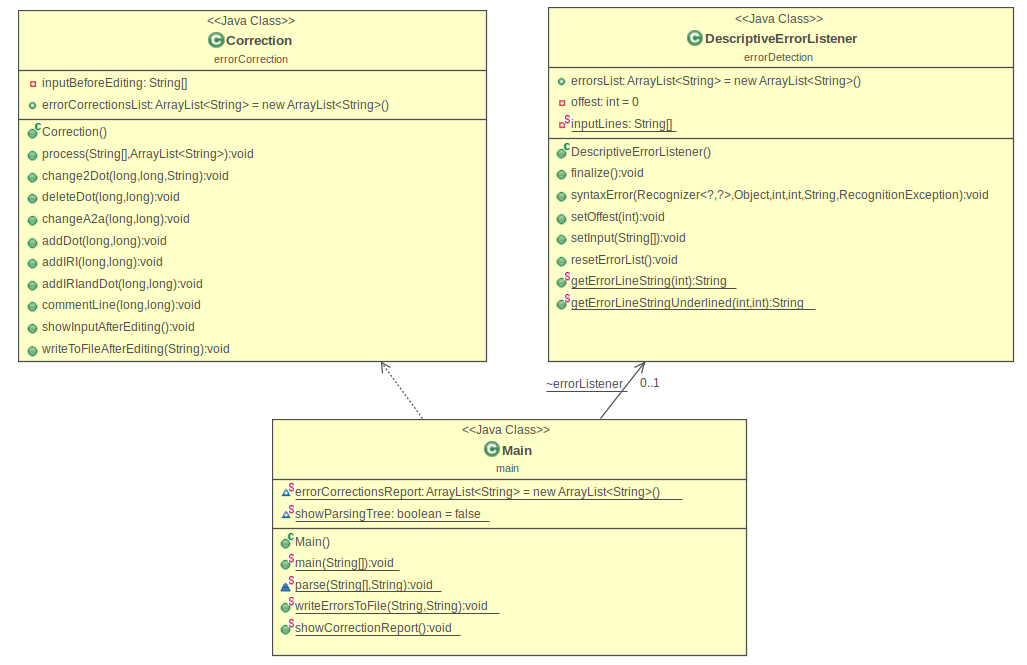
\includegraphics[scale=0.5,angle=0]{images/modules.png}
		\caption{UML diagram for the major modules in the proposed solution}
		\label{Fig:UML}
	\end{center}
\end{figure}

After briefing the proposed solution architecture, It is the time to cover it in more details by shedding light onto those modules which represent the pillars of such solution. {Figure \ref{Fig:UML}} establishes a UML diagram for the most significant modules in this solution, represented into 3 modules: Main, Error Detection, and Error Correction. The following text discusses those modules plus Core module. It is worth to be noted that Core module is not shown in {figure \ref{Fig:UML}} to facilitate the understanding of the main modules, otherwise it would be complex, furthermore, Core is automatically generated module by ANTLR based on the given grammar, thereby few changes were coded in the module:  
 \begin{enumerate}[]
 \item \textbf {Core}: is automatically generated by ANTLR based on the grammar defined appendix \ref{ch:appendix}. It encloses the parsing classes such as Parser, Lexer, Error Collector, Parse Tree Creator.   
\item \textbf{Errors Detection}: listens to the generated error messages by the parser. conventionally, while parsing if the parser detects syntax errors it sends a detail of the error to an error listener if one was defined. This module translates the list of errors were collected by the error listener into a valuable information about the error, such as an error expressive message to express the actual found error, an error location, identified by line and column numbers, and sometimes the actual line text where the parser has disclosed that error.
\item \textbf {Error Correction}: corrects those syntax errors which have only a well-know solution, this module was codded. The error message plays an important role to identify whether it can such error can be corrected or not. A global list stores all detected syntax errors messages and their location in the input (line number and column number) and this modules has predefined messages. if any of the detected error message matches any of the predefined messages, then such error can be healed and recovered.
\item \textbf{Main}: is the executive part which combines input, output, and processing components. It receives the input text, and if it is large (for example, more than 1 million lines), it is segmented into one or more chunks based on its size. Each chunk is handled separately in regards of parsing, error detection, as well as in error correction.

\end{enumerate} 

%TODO:check here how to adjust the vertical space 
\vspace{-5mm}

\section{Real-World Use Cases}
In this section, some of use cases tackled in this study to detect syntax errors in RDF input and  the method of error correction of some of those detected syntax error will be exposed. As a start, let's begin with a Turtle example which has no syntax errors, then some syntax errors can be introduced to show the process of handling them. 
	\vspace{5mm} %5mm vertical space

Listing \ref{lst:turtleExample} shows a Turtle example without syntax errors. First 4 lines are directives or prefixes declaration, rest of lines are triples.  For that reason, our grammar in appendix \ref{ch:appendix} was initialized with the topmost node \textbf{start}  which describes the coming rules by zero or more  \textbf{statement}(s). In addition, each \textbf{statement} is either a directive or a triple as it is represent in \ref{lst:startingRules}.

\begin{lstlisting}[label=lst:startingRules, caption={Starting rules in the grammar file}] 
start
: statement*  EOF
;
statement
: directive
| triples '.'
\end{lstlisting}

\begin{lstlisting}[label=lst:turtleExample, numbers=left, caption={RDF example in Turtle serialization format}]
<@\textcolor{blue}{@prefix}@>  <@\textcolor{red}{rdf}@>: <@\textcolor{orange}{<http://www.w3.org/1999/02/22-rdf-syntax-ns#>}@> .
<@\textcolor{blue}{@prefix}@>  <@\textcolor{red}{rdfs}@>:  <@\textcolor{orange}{<http://www.w3.org/2000/01/rdf-schema#>}@> .
<@\textcolor{blue}{@prefix}@>  <@\textcolor{red}{ex}@>:  <@\textcolor{orange}{<http://example.org/>}@> .
<@\textcolor{blue}{@prefix}@>  <@\textcolor{red}{zoo}@>:   <@\textcolor{orange}{<http://example.org/zoo/> }@> .
<@\textcolor{red}{ex}@>:dog1  <@\textcolor{red}{rdf}@>:type  <@\textcolor{red}{ex}@>:animal .
<@\textcolor{red}{ex}@>:cat1  <@\textcolor{red}{rdf}@>:type  <@\textcolor{red}{ex}@>:cat ;
         <@\textcolor{red}{rdfs}@>:label   <@\textcolor{green}{"Lusi"@en}@> .
<@\textcolor{red}{ex}@>:cat  <@\textcolor{red}{rdfs}@>:subClassOf  <@\textcolor{red}{ex}@>:animal .
<@\textcolor{red}{zoo}@>:host  <@\textcolor{red}{rdfs}@>:range  <@\textcolor{red}{ex}@>:animal .
<@\textcolor{red}{ex}@>:zoo1  <@\textcolor{red}{zoo}@>:host  <@\textcolor{red}{ex}@>:cat2 .
\end{lstlisting}



\begin{figure}

	\begin{subfigure}[]{}
		\centering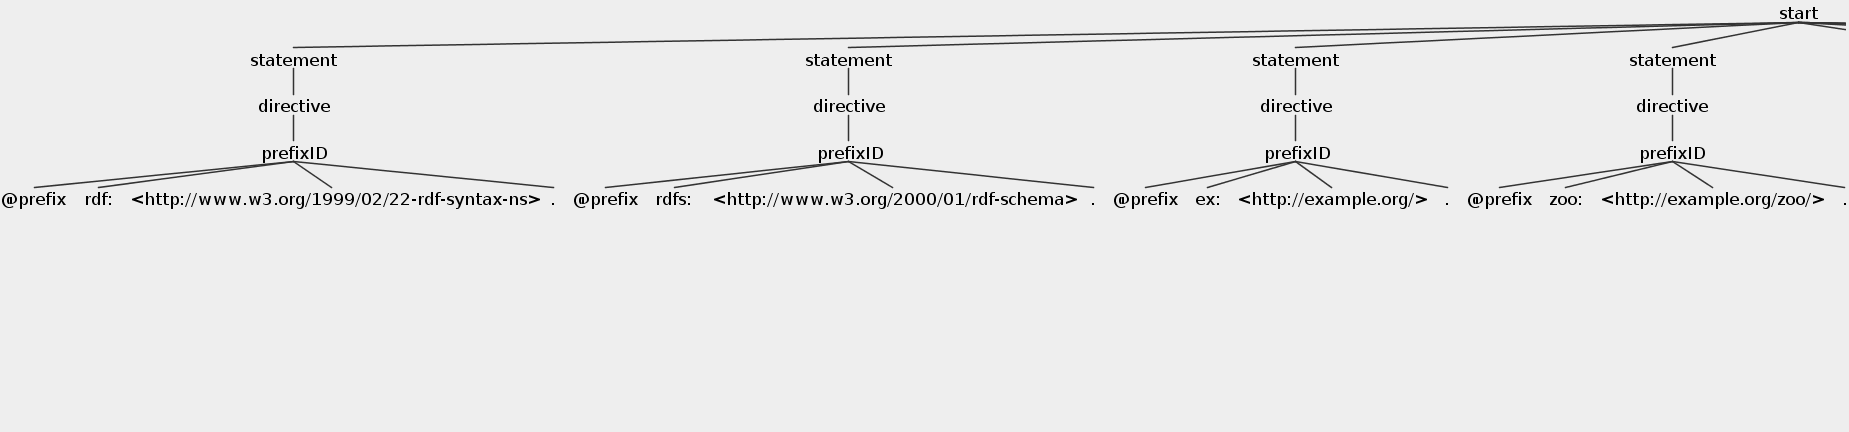
\includegraphics[width=1\linewidth]{images/parseTreeAllLeft.png}
	\end{subfigure}     
		\centering
	\begin{subfigure}[]{}
		\centering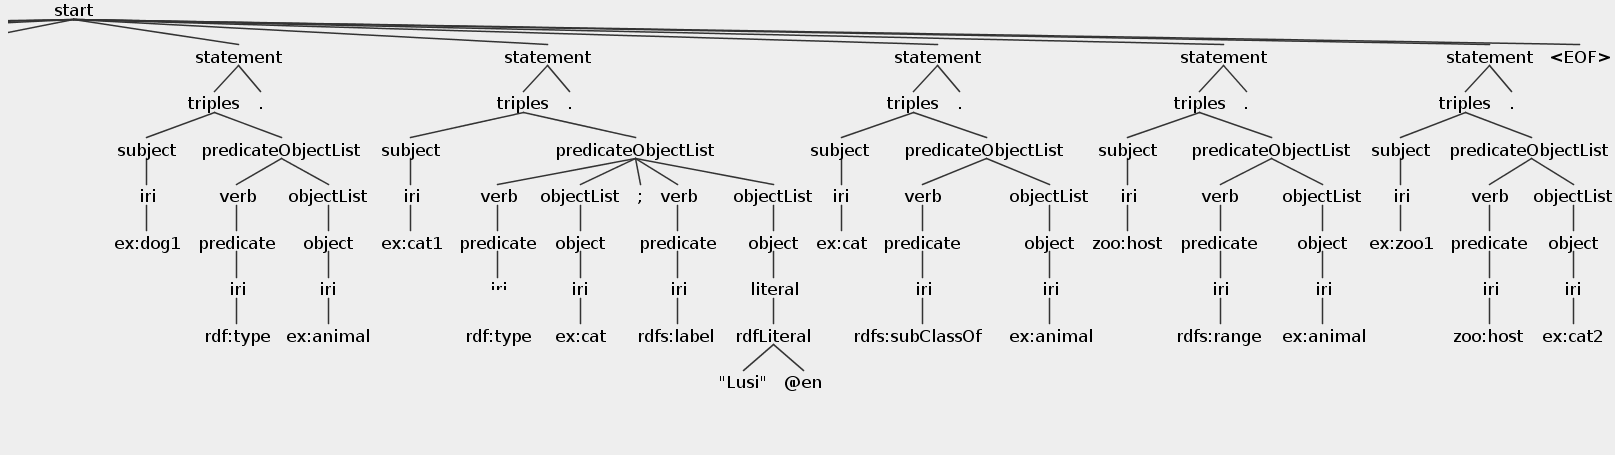
\includegraphics[width=1\linewidth]{images/parseTreeAlRight.png}
		\label{fig:rightSideParseTree}
	\end{subfigure}
	\caption{The parse tree view of listing \ref{lst:turtleExample}. (a) shows the left-side tree and (b) is the right-side tree. Both (a) and (b) are siblings of the parent node \textbf{start} in the parse tree  }
	\label{Fig:parseTreeTAll}
\end{figure}

After showing up a part of grammar rules and views of the parse tree, some of real cases of handling error detection and error recovery will be presented:
\begin{enumerate}
    \item \textbf{Missing a dot at the end of a triple:} in Turtle syntax, a triple must ends with a dot. In listing \ref{lst:missingDotEx}, the head rule \textbf{statement} as it was previously described, can be either directives or triples (ends with a dot). Equally important the last line which shows that triples without a dot can be also a sub-goal of this rule. This sub-goal is considered as a normal path in a parse tree, but, once the parser detects it, it sends a notifications to the error listener with an error message "Missing  ’.’ at the end of a triple".  
    
    
    \begin{lstlisting}[label=lst:missingDotEx,  caption={Detection of a syntax error of a missing dot at the end of a triple in the grammar }] 
statement
: directive
| triples '.'
| <@\textcolor{red}{triples  \{notifyErrorListeners("Bad end of a triple
               with ','")\} }@>;
\end{lstlisting}
Once such errors saves by the error listener, the role of Error Detection Module is finished. The next is the role of Error Correction Module to correct the error. Since the list of syntax error is shared with Error Correction Module, it iterates all of these errors messages, If one of these messages in the error list matches those which it includes, then it applies the predefined function.  For instance, \textbf{addDot(lineNum, columnNum)} function is applied in our case, as it is coded in listing \ref{lst:errorCorrectionlst}, since it matches the same error message and similarly, in case of "Missing  ’.’ at the  end of  Prefix directive" message. The activity of this function just to reach the line which misses the dot by the sent lineNum and columNum values and then adds a dot. 
    \begin{lstlisting}[language=java, label=lst:errorCorrectionlst,  caption={Java-based handling of error correction based on the error message in Error Correction Module }] 
while (iterator.hasNext()) {
String line = iterator.next();
// select the action based on the error message
if (line.contains("Missing '.' at the end of Prefix
directive")||line.contains("Missing '.' at the end 
of a triple"))
<@\textcolor{violet}{addDot(lineNum, columnNum);}@>
else if (line.contains("'A' cannot be used as
predicate, it should be repalced with 'a'"))
<@\textcolor{violet}{changeA2a(lineNum, columnNum);}@>
}
\end{lstlisting}

    \item \textbf{Misuse of 'A'  as a predicate instead of 'a':} by mistake a user can missuse of 'A' as a predicate instead of using 'a' (which is rdf:type, to ease its usage, it was replaced with 'a'). if we start substitution of sub-goals of triples, \textbf{verb} can be found as a terminal node in  substitution chain. syntactically, it is 'a', but if the user used 'A', then the parser will fire an error with a message "’A’ cannot be used as a predicate, it should be replaced with ’a’" 
    
    	\vspace{5mm} %5mm vertical space

    listing \ref{lst:errorCorrectionlst} also shows the handling of this error by executing \textbf{changeA2a(lineNum, columnNum)} function where the same error message is as well matched. This functions can access Turtle input with the referred lineNum and columNum, then it replaces 'A' with 'a' to correct that error. 
    	\vspace{5mm} %5mm vertical space

    \begin{lstlisting}[label=lst:MissuseAex ,  caption={Detection a syntax error of misuse of 'A' as a predicate instead of 'a' in the grammar}] 
statement
: directive
| triples '.';
triples
: subject predicateObjectList;
predicateObjectList
: verb objectList (';' (verb objectList)?)*;
verb
:'a'
| <@\textcolor{red}{'A' {notifyErrorListeners("'A' cannot be used as
predicate, it should be replaced with 'a'");}}@>;
\end{lstlisting}
\item \textbf{Bad syntax of a language tag in a literal:} 
Turtle formats has the ability to specify the language of literal (which can be only placed as an object) by the character '@' followed by alphabetic characters, for example, "en", "fr", "de" are tags for English, French, German languages simultaneously. \textbf{"cat"@en}, and \textbf{"Katze"@de} are samples of literals with using of language tags.
\begin{lstlisting}[label=lst:badlaguageTag,  caption={Starting rules in the grammar file8}] 
triples
: subject predicateObjectList;
predicateObjectList
: verb objectList (';' (verb objectList)?)*;
objectList
: object (',' object)*
object
: literal;
literal
: rdfLiteral;
rdfLiteral
: String (LANGTAG | '^^' iri)?
| <@\textcolor{red}{ String  BAD\_LANGTAG\_AS\_NUMBER  {notifyErrorListeners("Language tag cannot be a numeric value");} }@>;
BAD_LANGTAG_AS_NUMBER : 
'@' [0-9]+;
\end{lstlisting}

 Perhaps a user wants to states a language tag for a literal but a number instead of an alphabetic character was given such as \textbf{"cat"@1}, then this should be considered as a syntax error in Turtle format. Listing \ref{lst:badlaguageTag} handles the sequence of rules in the grammar to make a parser firing a syntax error when such state was encountered. It can be easily following the hierarchy stricture of the rules, starting with \textbf{triples} head rule till reaching the last two lines which explain that an RDF literal can be a string followed by BAD\_LANGTAG\_AS\_NUMBER (which '@' character followed by numbers). When the parser finds such pattern in the input it delivers a syntax error to the error listener. Unfortunate, no error correction can be applied here, since what the user meant is totally unknown to us.     
\end{enumerate}

\chapter{Evaluation}
\label{ch:evaluation}
To evaluate RDF-Doctor, firstly, it was tested against standard test cases, including formats of correct and incorrect syntax in files, secondly, to get rid of bias, a random number of errors was generated using Poisson distribution and uniform random number generators for a period of time of 8 hours to simulate a couple of syntax errors, produced by an ontology user, lastly, the performance of RDF-Doctor was measured when both the number of errors and the volumes of ontologies are varied. This chapter discusses all of such experiments in the following text. 
\section{Implementation}
Experiments were run on a Linux
Ubuntu 18.04 machine with a 4th Gen Intel Core i5-
4300U CPU, 3MB Cache, 2.90GHz with 8GB RAM
1333MHz DDR3. RDF-Doctor was implemented using
Java version 9. ANTLR framework version 4.7.1 was used to build the internal parser in RDF-Doctor, as well, as an imported library for compiling and running of it.  

In the following sections, 3 experiments to evaluate RDF-Doctor are presented. Each section handles an experiment by exploring its objective, presenting its procedure, and finally, ending with demonstration and discussion of the  result.   

\section{Validating with RDF Suite Test} In this experiment, RDF-Doctor was validated against RDF Suite Test, specifically Turtle serialization. Next text discusses the objective, shows the procedure, and finally, presents and discusses the result.     
\subsection{Objective}
The evaluation phase starts with \cite{TurtleTests:Online} where Test Suite files of Turtle serialization are found. There are multiple Test Suites for each of RDF serializations, recommend by W3 Consortium\footnote{https://www.w3.org/}. The proficiency of a parser for a certain serialization can be validated with these files found in a corresponding Test Suite. Therefore, the target of this experiment is to measure the proficiency of RDF-Doctor while testing with W3C Turtle Test Suite.

\subsection{Procedure}
Files at \cite{TurtleTests:Online} were prompted to validate a parser that parses a Turtle serialization, hence, it was used to test RDF-Doctor. Metrics of the experiment are both Precision and Recall, donated by equation \ref{eq:1} and \ref{eq:1} sequentially. The former measures the percentage of errors which correctly flagged as syntax errors, while the latter calculates the percentage of actual syntax errors which correctly recognized. Total number of files at \cite{TurtleTests:Online} is 275, divided to parts: files include  correct syntaxes; and files contain incorrect syntaxes, the latter is represented with 65 files, and the remaining are related to the former, as demonstrated by Table \ref{tab:TurtleSuit}. 
 
\begin{table}[]
\centering
\begin{tabular}{|l|l|l|l|}
\hline
\begin{tabular}[c]{@{}l@{}}Error Type Classification \end{tabular} & Detected & \begin{tabular}[c]{@{}l@{}}Not detected\end{tabular} & Total \\ \hline
 Escape Characters              &      0    &    4 &   4  \\ \hline
 Bad Keywords             &      5   &    0 &   5  \\ \hline
 Bad Literals with langTag             &      2   &    0 &   2  \\ \hline
 Bad Local Name-space in IRI             &      2   &    3  &   5  \\ \hline
 Bad Namespace in IRI             &      2   &    0 &   2  \\ \hline
 N3 Extra             &      11   &    1 &   12  \\ \hline
 Bad Namespace in Directives             &      2   &    0 &   2  \\ \hline
 Bad Number as a Literal             &      5   &    0 &   5  \\ \hline
 Bad Directives             &      4   &    0 &   4  \\ \hline
 Bad Strings             &      6   &    1 &   7  \\ \hline
 Bad Structures            &      12   &    0 &   12  \\ \hline
 Bad IRI            &      2   &    3 &   5  \\ \hline
 Total            &      53   &    12 &   65  \\ \hline
\end{tabular}
\caption{\textbf{Evaluation of RDF-Doctor against detection of incorrect syntactic forms in Turtle Test Suite \cite{TurtleTests:Online}.} The test focuses on the files, including  an incorrect Turtle syntax,  ”Detected” in pointed to recognized syntactic forms as incorrect forms with releasing corresponding error messages, but ”Not detected” specifies incorrect syntactic forms which are not recognized and might generate false positives.}
\label{tab:detection}
\end{table}

\subsection{Result and Discussion}

The test drives the result when dealing with either correct or incorrect Turtle syntax. Thus, correct syntaxes should be recognized as correct, similarly in case of incorrect syntaxes plus exception errors should be fired.  However,  the test result in Table \ref{tab:TurtleSuit} shows recognizes mostly of correct syntaxes with 88\%, while the remaining 12\% RDF-Doctor are not recognized and it consider them as errors. In the meanwhile, when dealing with incorrect syntaxes, again, Table \ref{tab:TurtleSuit} provides that 81,5\% of files included incorrect syntaxes are detected and an error message was fired for each one of them, the rest 17,5\% go without being identified as incorrect forms, as well as no errors were fired.



\begin{table}[]
\centering
\begin{tabular}{|l|l|l|l|}
\hline
\begin{tabular}[c]{@{}l@{}}File Content \end{tabular} & Detected  & Not detected & Total \\ \hline
 Correct Syntax              &      185    &      25  & 210 \\ \hline
 Incorrect/Bad Syntax              &      53    &    12  & 65 \\ \hline
 Total            &      238   &       37 & 275  \\ \hline
\end{tabular}
\caption{\textbf{Evaluation summary of RDF-Doctor for both correct and incorrect syntactic forms when validating with Turtle Test Suite \cite{TurtleTests:Online}.} "Detected" for Correct Syntax means that RDF-Doctor is able to recognize them as correct syntactic forms, whereas, for those which are not correctly recognized classified under "Not detected", similarly, "Detected" in Incorrect/Bad Syntax referred to recognized syntactic forms  as incorrect forms with releasing corresponding error messages, but "Not detected" specifies  incorrect syntactic forms  which are not recognized and might generate false positives.}
\label{tab:TurtleSuit}
\end{table}
\begin{figure}[ht]
\begin{center}
		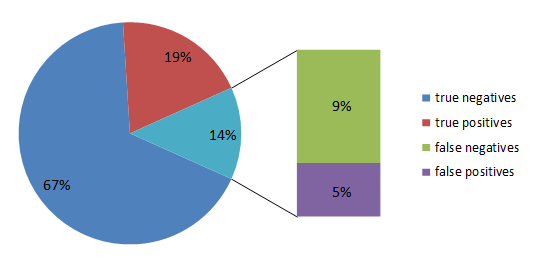
\includegraphics[scale=0.7,angle=0]{images/Experiment01.png}
		\caption{\textbf{RDF-Doctor evaluation with Turtle Test Suite \cite{TurtleTests:Online}.} Each file in \cite{TurtleTests:Online} was classified of having a syntax error or not and then the final result was grouped into 4 categories: true positives (files with syntax errors are correctly identified); false positives (files without syntax errors are incorrectly identified); false negatives (files with syntax errors are incorrectly rejected); true negatives (files without syntax errors are correctly rejected).}
		\label{Fig:Experiment01}
\end{center}
\end{figure}

For evaluation, the precision and recall are computed using the equations \ref{eq:1} and \ref{eq:2} respectively.  
\begin{align} 
   Precision=  \frac{t_p}{t_p+f_p}\,;\qquad
\qquad\parbox{4.0cm}{\footnotesize$\begin{aligned} t_p &= \text{ number of true positives}\\[-1.0ex] f_p &= \text{ number of false positives}\end{aligned}$}
   \label{eq:1}
\end{align}
\begin{align}
   Recall =  \frac{t_p}{t_p+f_n} \,;\qquad
\qquad\parbox{4.0cm}{\footnotesize$\begin{aligned} t_p &= \text{ number of true positives}\\[-1.0ex] f_n &= \text{ number of true negatives}\end{aligned}$}
   \label{eq:2}
\end{align}



\section{Validating with Random Syntax Errors Generation}
RDF-Doctor is being validated with injected syntax errors in random. What follows is a details of this experiment.
\subsection{Objective}
To get rid of the generated bias, this experiment uses both Poisson distribution and uniform random number generation methods. It also assumes a naive user editing an RDF input data, found in an environment similar to the one in Figure \ref{Fig:Motivation} and he is mistakenly generating some  syntax errors. Then, the inserted syntax errors evaluate the quality of RDF-doctor.


\subsection{Procedure}
 In this experiment, a naive user who is working on on RDF input data for 8 hours and each one hour he is making a text change (insert/modify/delete) before submission to RDF-Doctor for parsing is simulated. The average number of making syntax errors per time interval is represented by a parameter $\lambda$. For example, if   $\lambda$ = 5, it means that five syntax errors are occurred per hour.  As an input for a Poisson distribution, 10 syntax errors per instance of time was supplied. Hence, for each instance of time we calculate value of $\lambda$, then the output value drives how many number of syntax errors are entitled for that instance of time.
 
 Next, Those syntax errors are arbitrarily selected from the type of errors range [1-61], drawn by rows of Table \ref{tab:syntaxErrorCate}. Beside locations of injected syntax errors were controlled in a semi-random method, using the uniform random number generation to get a suggested line number if this location can be a correct location for such an error, otherwise, it can be nearby of the suggested line number on the top lines of the input file, such as Prefix and Base directives.   

\subsection{Result and Discussion}



	\begin{figure}[ht]
	\begin{center}
		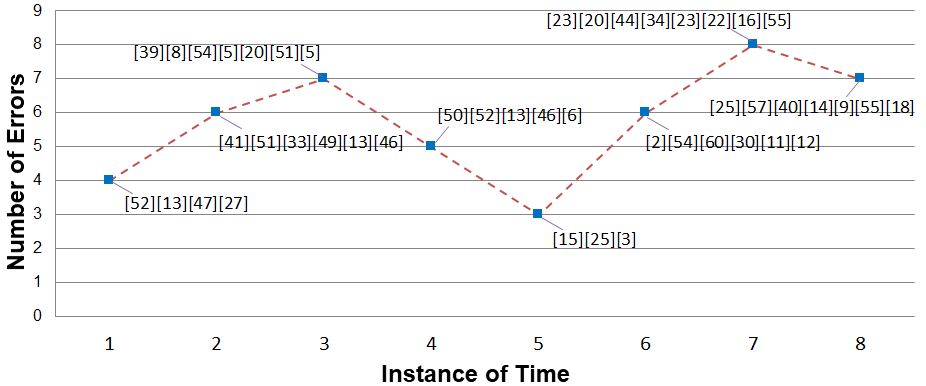
\includegraphics[scale=0.45,angle=0]{images/Experiment02-01.png}
		\setlength\belowcaptionskip{-5mm}
		\caption{\textbf{Random syntax errors distribution.} Number and types of syntax errors between brackets for a user in an interval of 8 instances of time. A Poisson  distribution with $\lambda$ = 5 models an average of 5 syntax errors per instance of time. Each instance of time shows value of $\lambda$, assuming the user can generate [1-10] syntax errors per instance of time. Also, a uniform random number generator computes type of errors from [1-61] syntax errors in Table \ref{tab:syntaxErrorCate}. For example, at the 5\textsuperscript{th} instance of time, $\lambda$ = 3, then 3 types of syntax errors are randomly generated.} 
		\label{Fig:experiment2}
	\end{center}
\end{figure}



	\begin{figure}[ht]
	\begin{center}
		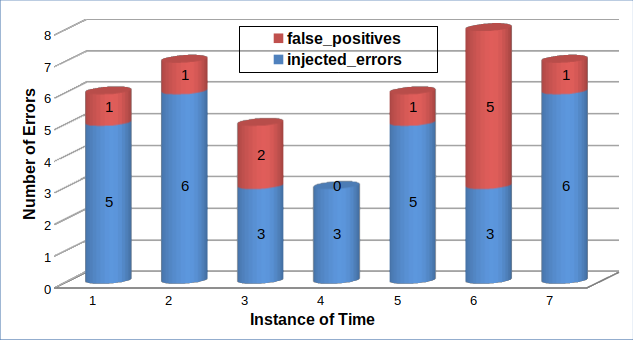
\includegraphics[scale=0.7,angle=0]{images/Experiment02-02.png}
		\setlength\belowcaptionskip{-5mm}
		\caption{\textbf{RDF-Doctor evaluation of error detection when syntax errors are randomly distributed.} For every instance of time, result shows number of errors between the injected one which were correctly detected by RDF-Doctor with giving corresponding error messages, pointed with "detected", and those one which were undetected and unrecognized by RDF-Doctor, referred as "undetected".} 
		\label{Fig:Experiment02-02}
	\end{center}
\end{figure}

	\begin{figure}[ht]
	\begin{center}
		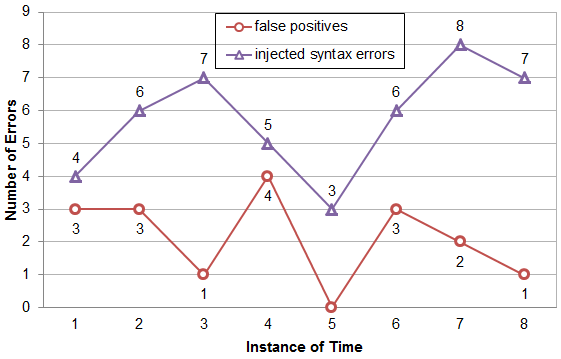
\includegraphics[scale=0.7,angle=0]{images/Experiment02-03.png}
				\setlength\belowcaptionskip{-5mm}

		\caption{\textbf{Result of False Positives during RDF-Doctor validating with randomly distributed syntax errors.} For each time instance, when number of syntax errors are inserted at random, that may result in false positives since one of the unrecognized syntax errors can be in-betweeen those inserted ones.} 
		\label{Fig:Experiment02-03}
				\setlength\belowcaptionskip{-5mm}
		\setlength\abovecaptionskip{0mm}
	\end{center}
\end{figure}

\section{Number of Errors and Volume Impact on Behaviour and  Performance of RDF-Doctor}
In last experiment, behaviour and  performance RDF-Doctor is being evaluated when a number of syntax errors and a volume of ontologies are changed. Details are shown in the following.  
\subsection{Objective}

In order to study the behaviour and the performance of RDF-Doctor, this experiment was performed. We are studying the effect of growing of number of syntax errors, as well as, the size of ontologies when it is changed. 


\subsection{Procedure}
Two types of ontologies are used: small; and medium size. For the former, FOAF  (an abbreviation form of friend of a friend) Vocabulary\footnote{http://www.foaf-project.org/} was used, it is a small ontology with volume of about 23.3 Kbyte, including people-related terms. Whilst the latter made use of the ontology  of DBpedia schema\footnote{https://wiki.dbpedia.org/develop/datasets/dbpedia-version-2016-10}, version 2016-10, with volume of about 4.1 Mbyte, including meta-data about all contained datasets of DBpedia. Both datasets were used 3 times and for one time 10, 30, 61 syntax errors were randomly  injected using the same procedure of uniform random generation. Additionally, to evaluate the performance of RDF-Doctor, same 6 of the datasets were parsed for 5 times to get the average of processing time  

 
\subsection{Result and Discussion}
Figure \ref{Fig:Experiment03-01} drives the impact of number of errors and the volume size. When introducing 10 syntax error, 9 out 10 were detected and one was not detected for both FOAF and DBpedia. 25 out 30 injected syntax errors in FOAF and 26 out 30 injected syntax errors in DBpedia were detected, the rest are undetected. Subsequently, 61 syntax errors were inserted 6 and 11 syntax errors go undetected in FOAF, DBpedia, respectively, the remaining are detected with expressive error messages to help users in resolving such errors. 
\begin{figure}[ht]
\begin{center}
		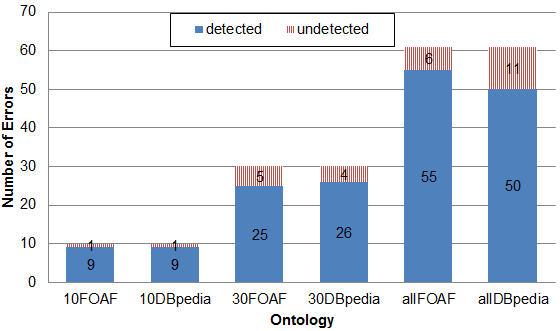
\includegraphics[scale=0.49,angle=0]{images/Experiment03-01.png}
				\setlength\belowcaptionskip{-5mm}

		\caption{\textbf{Impact of number of errors and volume on RDF-Doctor.} FOAF, and DBpedia ontologies were used to evaluate RDF-Doctor, 10foaf, 30foaf, allfoaf are datasets of FOAF ontology, including with 10, 30, 61 random syntax errors, respectively, same is applicable for DBpedia. Detected errors are the errors which were properly identified by RDF-Doctor and the matched error messages were released, while undetected errors are those which not correctly recognized.}
		\label{Fig:Experiment03-01}

\end{center}
\end{figure}


Another essential point is number of false positives were shown in the result, as it is demonstrated  by Figure \ref{Fig:Experiment03-02}. Clearly, it can be seen that the false positives  are incremented while raising of the number of syntax errors, that comes as consequence of increasing number of unrecognized syntax errors, then the parser tries to recover from such errors by adding or removing some tokens which produces more and more false positives.   




\begin{figure}[ht]
\begin{center}
		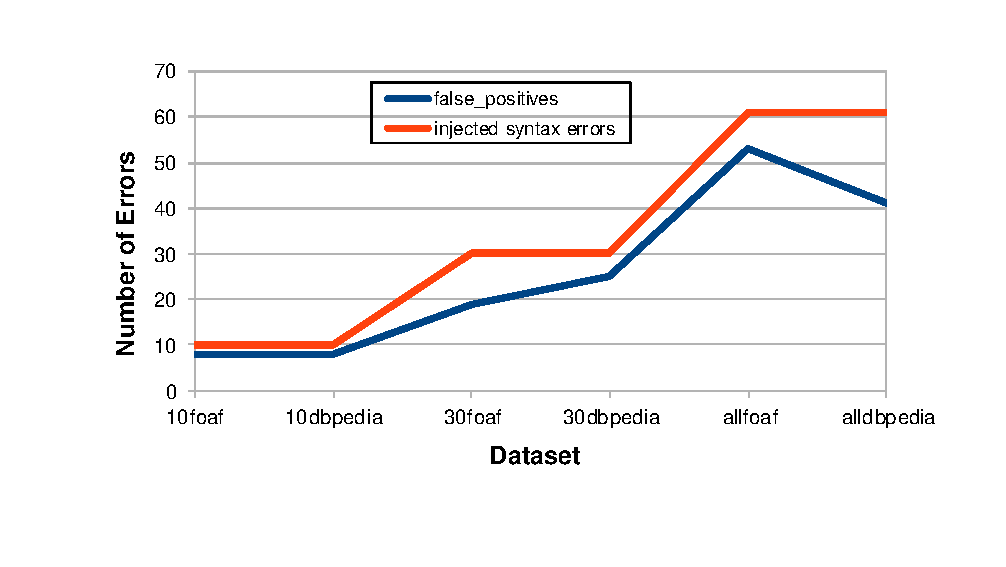
\includegraphics[scale=0.8,angle=0]{images/Experiment03-02.pdf}
		\setlength\belowcaptionskip{-5mm}
		\setlength\abovecaptionskip{-10mm}
		\caption{\textbf{Result of False Positives when number of errors and volume sizes are varied.} Undetected errors generate false-positive errors and when the number of errors increase, the false-positives are comparably increased.}
				\label{Fig:Experiment03-02}
\end{center}
\end{figure}

Due to the need to measure the RDF-Doctor performance, Figure \ref{Fig:Experiment03-03} was presented. it summaries the impact of both number of errors and volume on RDF-Doctor performance, where numbers of errors has no influence on the performance, as the processing time similar result in either FOAF or DBpedia while changing number of errors. In the meanwhile, volumes has a high impact on the performance, since  DBpedia  takes about 29000 ms in average to be processed, whereas, FOAF was parsed in about 2000 ms.   

To conclude this experiment, It can be seen that number of error detection is promising, more than 90\% of injected syntax errors were detected, as Figure \ref{Fig:Experiment03-01} talks. Also, number of false positives can be improved if RDF-Doctor recognized those undetected errors by either do more laboratory works to match those patterns or may with the new versions of ANTLR library.  
%talk about the correction of errors #numbers 
\begin{figure}[ht]
\begin{center}
		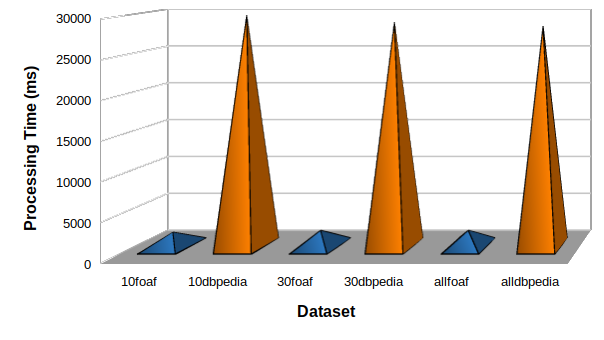
\includegraphics[scale=0.7,angle=0]{images/Experiment03-03.png}
		\setlength\belowcaptionskip{-5mm}
		\setlength\abovecaptionskip{0mm}
		\caption{\textbf{RDF-Doctor performance evaluation when number of errors and volume sizes are varied.} Performance is measured with the processing time in (ms) of FOFA ontology (23.3 Kbyte) and DBpedia ontology (4.1 Mbyte) with 10, 30, and 61 (refereed as all) injected syntax errors.}
				\label{Fig:Experiment03-03}

\end{center}
\end{figure}

\chapter{Conclusions and Future Work}
\label{ch:conclusions}
\newpage


%% ----------------------------------------------------------------
\clearpage
%------------------------------------------------------------------------------
\label{Bibliography}
\bibliographystyle{unsrtnat}  % Use the "unsrtnat" BibTeX style for formatting the Bibliography\bibliographystyle{plain}
\nocite{*}
\bibliography{literature}  % The references (bibliography) information are stored in the file named "Bibliography.bib"
\let\cleardoublepage\clearpage
\begin{appendices}
\chapter{RDF-Doctor Grammar}
\label{ch:appendix}
% Applies only when you use it
\lstset{
    basicstyle=\color{black}\ttfamily,%
    breaklines=true,%                                      allow line breaks
    moredelim=*[s][\color{black}\ttfamily]{options}{\}},%  options in black (until trailing })
    commentstyle={\color{gray}\itshape},%                  gray italics for comments
    morecomment=[l]{//},%                                  define // comment
    emph={%
        STRING%                                            literal strings listed here
        },emphstyle={\color{blue}\ttfamily},%              and formatted in blue
    alsoletter={:,|,;},%
    morekeywords={:,|,;},%                                 define the special characters
    keywordstyle={\color{black}},%                         and format them in black
}

\begin{lstlisting}
// title of the grammar
grammar Turtle;
// functions in Java as a target programming language for RDF-Doctor parser
@parser::members { 
// Add member functions to check a Namespace declaration
public List<String> symbols = new ArrayList<String>();
boolean isExistNS(String in ) { 
	boolean foundNS = false ; 
		if(symbols.contains(in.split(":")[0]+':')) foundNS=true;
	return foundNS;
}
}
// the beginning of the grammar rules with 'start' root node
start
    : statement*  EOF
    ;
// 'statement' is a rule for either a triple or a prefix
statement
    : directive
    |  IRIREF IRIREF IRIREF  graphLabel '.'
// 'notifyErrorListeners' is a function to announce the existence of an error with its corresponding error message, same is applied for next rules
    {notifyErrorListeners("Turtle is not NQOUDS");}
    | triple '.'
    | triple {notifyErrorListeners("Missing '.' at the end of a triple");}
    | triple ',' {notifyErrorListeners("Bad end of a triple with ','");}
    | triple ';' {notifyErrorListeners("Bad end of a triple with ';'");}
    | triple ('.')+ ('.')+ {notifyErrorListeners("Too many DOT");}
    | errors		
    ;
// 'directive' is a rule for either a base or a prefix declaration
directive
    : sparqlPrefix
    | sparqlBase 
    | prefixID   
    | base
    | unkonwnDecl
    | sparqlPrefix '.' {notifyErrorListeners("Extraneous '.' at the end of SPARQL prefix directive");}
    | sparqlBase '.' {notifyErrorListeners("Extraneous '.' at the end of SPARQL base directive");}
    ;
// a rule to match certain incorrect syntax patterns
errors	
    : iri '=' iri '.' {notifyErrorListeners("'=' sign cannot be used in Turtle");}
 	| iri '<=' iri '.'  {notifyErrorListeners("'<=' symbol cannot be used in Turtle");}
    | iri '=>' iri '.'  {notifyErrorListeners("'=>' symbol cannot be used in Turtle");}
 	| (iri '.')+ (iri '.')+  triple '.' {notifyErrorListeners("N3 paths cannot be used in Turtle");}
    | (iri '.')+ (iri '.')+  triple  {notifyErrorListeners("N3 paths cannot be used in Turtle");}
    | iri '^'  triple '.' {notifyErrorListeners("N3 paths cannot be used in Turtle");}
    | '@forAll' iri '.' {notifyErrorListeners(" '@forAll' cannot be used in Turtle ");}
    | '@forSome' iri '.' {notifyErrorListeners(" '@forSome' cannot be used in Turtle ");}
    | ('a'|CHARS)* '@a' ('a'|CHARS)* '.' {notifyErrorListeners(" '@a' cannot be used in Turtle ");}
    ;
 graphLabel
 	: 	IRIREF | BLANK_NODE_LABEL
 	;
 unkonwnDecl 	
    : '@keywords' ('a'|CHARS)*  '.' {notifyErrorListeners("@keywords is unkown directive in Turtle");}
	;
// a rule for a prefix declaration to match  correct and incorrect forms
prefixID
    : '@prefix' CHARS '.' ':' IRIREF '.' {notifyErrorListeners("Prefix-label cannot end with '.' ");}
    | '@prefix' '.' CHARS ':' IRIREF '.' {notifyErrorListeners("Prefix-label cannot start with '.' ");}
    | '@prefix' ':' IRIREF '.' { symbols.add(":");} { System.out.println(":" + $IRIREF.text);} 
    | '@prefix' PNAME_NS  IRIREF '.' {symbols.add($PNAME_NS.text);}  { System.out.println($PNAME_NS.text + $IRIREF.text);} 
    | '@prefix' PNAME_NS IRIREF ('.')+ ('.')+ {notifyErrorListeners("Too many DOT ");}
    | PNAME_NS IRIREF '.' {notifyErrorListeners("Missing Prefix keyword, use '@prefix'");}
    | '@prefix'   IRIREF '.' {notifyErrorListeners("Missing Prefix-label in Prefix directive");}
    | '@prefix' CHARS*  IRIREF '.'  {notifyErrorListeners("Missing ':' in Prefix directive");}
    ;
// a rule for a base declaration to match  correct and incorrect forms
base
    : '@base' IRIREF '.'
    | '@base' IRIREF ('.')+ ('.')+ {notifyErrorListeners("Too many DOT ");}
    ;
sparqlBase
    : KW_BASE  IRIREF 
    | '@BASE'   IRIREF '.'  {notifyErrorListeners("incorrect syntax form of base directive");}
    ;
sparqlPrefix
    : KW_PREFIX CHARS '.' ':' IRIREF  {notifyErrorListeners("Prefix-label cannot end with '.' ");}
    | KW_PREFIX '.' CHARS ':' IRIREF  {notifyErrorListeners("Prefix-label cannot start with '.' ");}
    | KW_PREFIX PNAME_NS IRIREF
    | KW_PREFIX ':' IRIREF
    | PNAME_NS IRIREF {notifyErrorListeners("Missing Prefix keyword, use 'PREFIX'");}
    | KW_PREFIX  IRIREF  {notifyErrorListeners("Missing Prefix-label in Prefix directive");}
    ;
// declare keywords
KW_BASE 
    : B A S E 
    ;
KW_PREFIX 
    : P R E F I X 
    ;
// rules for a triple with correct and incorrect forms
triple
    : subject predicateObjectList
    | blankNodePropertyList predicateObjectList?
    | subject ':' object 
    | subject verb {notifyErrorListeners("Object of a triple is missing");}
    ;
predicateObjectList
    : verb objectList (';' verb objectList)*
    | verb objectList (';' verb objectList)* ('.')+ {notifyErrorListeners("Too many dots ");}
    | verb objectList (';' verb )* {notifyErrorListeners("Object of a triple is missing");}
    | verb  (';' verb objectList)* {notifyErrorListeners("Object of a triple is missing");}
    | verb objectList (';' verb objectList)* (';' verb )+ (';' verb objectList)* {notifyErrorListeners("Object of a triple is missing");}
    ;
objectList
    : object (',' object)*
    ;
// a rule for a predicate in a triple with correct and incorrect forms
verb
    :   'a' 
    | predicate
    | 'is' predicate 'of' {notifyErrorListeners("'is .. of' pattern is not used in Turtle");}
    | 'A' {notifyErrorListeners("'A' cannot be used as predicate, it should be replaced with 'a'");}
    | BooleanLiteral {notifyErrorListeners("Predicate cannot be a Boolean value");}
    | NumericLiteral  {notifyErrorListeners("Predicate cannot be a number");}
    | literal {notifyErrorListeners("Predicate cannot be a literal");}
    | BlankNode {notifyErrorListeners("Predicate cannot be a blank node");}
    ;
// a rule for a subject in a triple with correct and incorrect forms
subject
    : iri
    | BlankNode
    | BlankNode  '.' {notifyErrorListeners("Blank Node cannot be followed by '.'");}
    | 'a' {notifyErrorListeners("'a' cannot be used as a subject");}
    | BooleanLiteral {notifyErrorListeners("Subject cannot be a Boolean value");}
    | NumericLiteral  {notifyErrorListeners("Subject cannot be a number");}
    | rdfLiteral   {notifyErrorListeners("Subject cannot be a string");}
    | collection
    | '{' triple '.' '}' {notifyErrorListeners("{ } pattern cannot be used in Turtle");}
    | '{' triple '}' {notifyErrorListeners("{ } pattern cannot be used in Turtle");} 
    ;
predicate
    : iri
    ;
// a rule for an object in a triple with correct and incorrect forms
object
    : iri
    | BlankNode
    | collection
    | blankNodePropertyList
    | badBlankNodePropertyList  {notifyErrorListeners("incorrect form of a blank node list");}
    | literal
    | 'a' {notifyErrorListeners("'a' cannot be used as an object");}   
    ;
// a rule for literal replacing an object  with correct and incorrect forms
literal
    : rdfLiteral
    | NumericLiteral
    | BooleanLiteral
    | BadLiteral {notifyErrorListeners("incorrect form of a Literal");}
    ;
blankNodePropertyList
    : '[' predicateObjectList ']'
    ;
badBlankNodePropertyList   
	: '[' predicateObjectList '.' ']'
	;
collection
    : '(' object* ')'
    ;
NumericLiteral
    : INTEGER | DECIMAL | DOUBLE
    ;
rdfLiteral
    : BAD_STRING_LITERAL_LONG_QUOTE_WITH_OPEN_QUOTES  (LANGTAG | '^^' iri)?  {notifyErrorListeners("incorrect form of long literal with uncolsed qoutes");}
    | BAD_STRING_LITERAL_LONG_QUOTE_TOO_MANY (LANGTAG | '^^' iri)? {notifyErrorListeners("incorrect form of long literal with 4 qoutes");}
    | BAD_STRING_LITERAL_LONG_SINGLE_QUOTE_TOO_MANY (LANGTAG | '^^' iri)? {notifyErrorListeners("incorrect form of long literal with 4 qoutes");}
    | String  BAD_LANGTAG_AS_NUMBER  {notifyErrorListeners("Language tag cannot be a numeric value");}
    | String '^' iri {notifyErrorListeners("Missing '^' Character");}
    | String LANGTAG '^^' iri {notifyErrorListeners("incorrect form of a Literal");}
    | String '^^' iri LANGTAG {notifyErrorListeners("incorrect form of a Literal");}  
    | (BAD_STRING_LITERAL_LONG_SINGLE_QUOTE | BAD_STRING_LITERAL_LONG_QUOTE ) (LANGTAG | '^^' iri)?  {notifyErrorListeners("incorrect quotes of a literal");}
    | BAD_STRING_LITERAL_SINGLE_QUOTE (LANGTAG | '^^' iri)? {notifyErrorListeners("incorrect quotes of a literal");}
    | BAD_STRING_LITERAL_QUOTE (LANGTAG | '^^' iri)? {notifyErrorListeners("incorrect quotes of a literal");}
    | (BAD_STRING_LITERAL_QUOTE_WITH_BAD_UCHAR | BAD_STRING_LITERAL_SINGLE_QUOTE_WITH_BAD_UCHAR | BAD_STRING_LITERAL_LONG_SINGLE_QUOTE_WITH_BAD_UCHAR | BAD_STRING_LITERAL_LONG_QUOTE_WITH_BAD_UCHAR) {notifyErrorListeners("Bad Unicode Characters, Only HEX Characters are allowed");}
    | (BAD_STRING_LITERAL_QUOTE_WITH_BAD_ESCAPE | BAD_STRING_LITERAL_SINGLE_QUOTE_WITH_BAD_ESCAPE | BAD_STRING_LITERAL_LONG_SINGLE_QUOTE_WITH_BAD_ESCAPE | BAD_STRING_LITERAL_LONG_QUOTE_WITH_BAD_ESCAPE) {notifyErrorListeners("Bad Literal Escape");}
    |  String (LANGTAG | '^^' iri)?
    ;
// a rule for BooleanLiteral which can be either true or false
BooleanLiteral
    : 'true' | 'false'
    ;
// a rule for incorrect literal patterns
BadLiteral 
    : NumericLiteral ('.')+ CHARS 
    | NumericLiteral CHARS 
    | '+' '-' NumericLiteral
    ;
String
    : STRING_LITERAL_QUOTE | STRING_LITERAL_SINGLE_QUOTE | STRING_LITERAL_LONG_SINGLE_QUOTE | STRING_LITERAL_LONG_QUOTE
    ;
// a rule for IRI to match either incorrect or correct patterns
iri
    : ':' BAD_PN_LOCAL_STARTS_WITH_TILDE {notifyErrorListeners("Bad syntax of Prefixed IRI, the local prefix namespace cannot contain '~'");}
    |    PN_LOCAL_BAD_WITH_DASH {notifyErrorListeners("Bad syntax of Prefixed IRI, the local prefix namespace cannot start with dash");}
    | PrefixedName {if (!isExistNS($PrefixedName.text)){ notifyErrorListeners($PrefixedName.text.split(":")[0] +": prefix in " + $PrefixedName.text + " is undefined");}}
    | IRIREF 
    | PN_PREFIX? ':'  BAD_PN_LOCAL_STARTS_WITH_PERCENT {notifyErrorListeners("Bad syntax of Prefixed IRI, the local prefix namespace cannot contain '%'");}
    | BAD_PNAME_LN_STARTS_WITH_DOT  {notifyErrorListeners("incorrect form of Prefix-label, it cannot start with '.'");} 
    | BAD_PNAME_LN_ENDS_WITH_DOT  {notifyErrorListeners("incorrect form of Prefix-label, it cannot end with '.'");} 
    | BAD_IRIREF_WITH_SPACE {notifyErrorListeners("Bad syntax of IRI, IRI cannot contain space or newline");}
    | BAD_IRIREF_WITH_MULTIPLE_ANGLE_BRACKETS {notifyErrorListeners("Bad syntax of IRI, Too many angle brackets in IRI");}
    | BAD_IRIREF_WITH_PARENTHESES {notifyErrorListeners("Bad syntax of IRI, IRI cannot contain unexpected characters");}
    ;
BlankNode
    : BLANK_NODE_LABEL 
    | ANON
    ;
// a rule to skip spaces, tabs and empty lines
WS
    : ([\t\r\n\u000C] | ' ') + -> skip
    ;
// a rule to skip comments starting with '#'
COMMENT				  
	: '#' ~[\r\n]* -> skip;
// LEXER rules
CHARS
    : [a-zA-Z]+ [0-9]*
	;
PN_PREFIX
    : PN_CHARS_BASE ((PN_CHARS | '.')* PN_CHARS)?
    ;
IRIREF
    : '<' (~[\u0000-\u0020<>"{}|^`\\] | UCHAR)* '>' 
    ;
PNAME_NS
    : PN_PREFIX? ':'
    ;
PrefixedName
    :  PNAME_NS | PNAME_LN
    ;
PNAME_LN
    : PNAME_NS PN_LOCAL 
    ;
BAD_PNAME_LN_STARTS_WITH_DOT	  
	 : '.' PN_PREFIX ':' PN_LOCAL 
	 ;
BAD_PNAME_LN_ENDS_WITH_DOT	  
	 : PN_PREFIX  '.:' PN_LOCAL 
	 ;
BLANK_NODE_LABEL
    : '_:' (PN_CHARS_U | [0-9]) ((PN_CHARS | '.')* PN_CHARS)?
    ;
LANGTAG
    : '@' [a-zA-Z] + ('-' [a-zA-Z0-9] +)*
    ;
BAD_LANGTAG_AS_NUMBER
    : '@' [0-9]+
    ;
INTEGER
    : [+-]? [0-9]+
    ;
DECIMAL
    : [+-]? [0-9]* '.' [0-9] +
    ;
DOUBLE
    : [+-]? ([0-9] + '.' [0-9]* EXPONENT | '.' [0-9] + EXPONENT | [0-9] + EXPONENT)
    ;
EXPONENT
    : [eE] [+-]? [0-9] +
    ;
STRING_LITERAL_LONG_SINGLE_QUOTE
    : '\'\'\'' (~[\u0027\u005C\u000A\u000D] | ECHAR | UCHAR  | '\n' )*  ('\'' | '\'\'')?  (~[\u0027\u005C\u000A\u000D] | ECHAR | UCHAR)* '\'\'\''  
    ;
STRING_LITERAL_LONG_QUOTE
    : '"""'  ((~ ["\\] | ECHAR | UCHAR | '\'') ('"' | '""')? (';'| ',' |'.')* (~ ["\\] | ECHAR | UCHAR | '\''))* '"""'
    ;
STRING_LITERAL_QUOTE
    : '"' (~[\u0022\u005C\u000A\u000D] | ECHAR | UCHAR)* '"' 
    ;
STRING_LITERAL_SINGLE_QUOTE
    : '\'' (~ [\u0027\u005C\u000A\u000D] | ECHAR | UCHAR | '"')* '\''
    ;
// rules for IRI to match incorrect forms 
BAD_IRIREF_WITH_SPACE
 	:  '<' (PN_CHARS | '.' | ':' | '/' | '\\' | '#' | '@' | '%' | '&' | UCHAR)* '\n>'
	| '<' (PN_CHARS | '.' | ':' | '/' | '\\' | '#' | '@' | '%' | '&' | UCHAR)* '\u0020>'
	| '<' (PN_CHARS | '.' | ':' | '/' | '\\' | '#' | '@' | '%' | '&' | UCHAR)* ANON_WS+ (PN_CHARS |'.' | ':' | '/' | '\\' | '#' | '@' | '%' | '&' | UCHAR)*'>'
	;
BAD_IRIREF_WITH_MULTIPLE_ANGLE_BRACKETS
	:'<' (PN_CHARS | '.' | ':' | '/' | '\\' | '#' | '@' | '%' | '&' | UCHAR)* '\u003C>'
	| '<' (PN_CHARS | '.' | ':' | '/' | '\\' | '#' | '@' | '%' | '&' | UCHAR)* '\u003E>'
	;
BAD_IRIREF_WITH_PARENTHESES 
    : '<' (PN_CHARS | '.' | ':' | '/' | '{'| '}' | '\\' | '#' | '@' | '%' | '&' | UCHAR)* '>'
	;
// rules for incorrect literals
BAD_STRING_LITERAL_SINGLE_QUOTE   
    : '\'\'\'' (~[\u0027\u005C\u000A\u000D] | ECHAR | UCHAR)* '\'' 
	| '\'' (~[\u0027\u005C\u000A\u000D] | ECHAR | UCHAR)* '\'\'\'' 
	;
BAD_STRING_LITERAL_QUOTE      
	: '"""' (~[\u0022\u005C\u000A\u000D] | ECHAR | UCHAR)* '"' 
	| '"' (~[\u0022\u005C\u000A\u000D] | ECHAR | UCHAR)* '"""' 
	| '"' (~[\u0022\u005C\u000A\u000D] | ECHAR | UCHAR)* '\'' 
	| '\'' (~[\u0022\u005C\u000A\u000D] | ECHAR | UCHAR)* '"' 	
	| '"''\'' (~[\u0022\u005C\u000A\u000D] | ECHAR | UCHAR)* '""' 			
	;  	  
BAD_STRING_LITERAL_LONG_SINGLE_QUOTE
	: '\'\'\'' (('\'' | '\'\'')? ([^'\\] | ECHAR | UCHAR | '"'))* '"""'
	;
BAD_STRING_LITERAL_LONG_QUOTE
	: '"""' (('"' | '""')? (~ ["\\] | ECHAR | UCHAR | '\''))* '\'\'\''
	|  '"""' (('"' | '""')? (~ ["\\] | ECHAR | UCHAR | '\''))* '"' '\''
	|  '"' '\'' (~ ["\\] | ECHAR | UCHAR | '\'')* '""'
	;
BAD_STRING_LITERAL_LONG_QUOTE_TOO_MANY
	: '"""'  (~ ["\\] | ECHAR | UCHAR )* '""""'
	| '""""' (('"' | '""')? (~ ["\\] | ECHAR | UCHAR ))* '"""' 
	;	
BAD_STRING_LITERAL_LONG_SINGLE_QUOTE_TOO_MANY
	: '\'\'\'' (~[\u0027\u005C\u000A\u000D] | ECHAR | UCHAR)*  '\'\'\'\''
	| '\'\'\'\''(~[\u0027\u005C\u000A\u000D] | ECHAR | UCHAR)*  '\'\'\''
	;
BAD_STRING_LITERAL_QUOTE_WITH_BAD_UCHAR
    : '"' (~[\u0022\u005C\u000A\u000D] | ECHAR | UCHAR)* BAD_UCHAR (~[\u0022\u005C\u000A\u000D] | ECHAR | UCHAR)* '"' 
    ;
BAD_STRING_LITERAL_SINGLE_QUOTE_WITH_BAD_UCHAR
    : '\'' (~ [\u0027\u005C\u000A\u000D] | ECHAR | UCHAR | '"')*  BAD_UCHAR (~ [\u0027\u005C\u000A\u000D] | ECHAR | UCHAR | '"')*  '\''
    ;
BAD_STRING_LITERAL_LONG_SINGLE_QUOTE_WITH_BAD_UCHAR
    : '\'\'\'' (~[\u0027\u005C\u000A\u000D] | ECHAR | UCHAR  | '\n' )*  ('\'' | '\'\'')?  (~[\u0027\u005C\u000A\u000D] | ECHAR | UCHAR)* BAD_UCHAR   (~[\u0027\u005C\u000A\u000D] | ECHAR | UCHAR  | '\n' )*  ('\'' | '\'\'')?  (~[\u0027\u005C\u000A\u000D] | ECHAR | UCHAR)*'\'\'\''  
    ;
BAD_STRING_LITERAL_LONG_QUOTE_WITH_BAD_UCHAR
    : '"""'  (~[\u0022\u005C\u000A\u000D] | ECHAR | UCHAR)*   BAD_UCHAR (~[\u0022\u005C\u000A\u000D] | ECHAR | UCHAR)*   '"""'
    ;
BAD_STRING_LITERAL_LONG_QUOTE_WITH_OPEN_QUOTES
    : '"""'  (~ ["\\] | ECHAR | UCHAR )* '\n' '\n'
    ;
BAD_STRING_LITERAL_QUOTE_WITH_BAD_ESCAPE
    : '"' (~[\u0022\u005C\u000A\u000D] | ECHAR | UCHAR)* ILLEGAL_ESCAPE (~[\u0022\u005C\u000A\u000D] | ECHAR | UCHAR)* '"' 
    ;
BAD_STRING_LITERAL_SINGLE_QUOTE_WITH_BAD_ESCAPE
    : '\'' (~ [\u0027\u005C\u000A\u000D] | ECHAR | UCHAR | '"')*  ILLEGAL_ESCAPE (~ [\u0027\u005C\u000A\u000D] | ECHAR | UCHAR | '"')*  '\''
    ;
BAD_STRING_LITERAL_LONG_SINGLE_QUOTE_WITH_BAD_ESCAPE
    : '\'\'\'' (~[\u0027\u005C\u000A\u000D] | ECHAR | UCHAR  | '\n' )*  ('\'' | '\'\'')?  (~[\u0027\u005C\u000A\u000D] | ECHAR | UCHAR)* ILLEGAL_ESCAPE   (~[\u0027\u005C\u000A\u000D] | ECHAR | UCHAR  | '\n' )*  ('\'' | '\'\'')?  (~[\u0027\u005C\u000A\u000D] | ECHAR | UCHAR)*'\'\'\''  
    ;
BAD_STRING_LITERAL_LONG_QUOTE_WITH_BAD_ESCAPE
    : '"""'  (~[\u0022\u005C\u000A\u000D] | ECHAR | UCHAR)*   ILLEGAL_ESCAPE (~[\u0022\u005C\u000A\u000D] | ECHAR | UCHAR)*   '"""'
    ;
// a rule for Unicode characters
fragment UCHAR
    : '\\u' HEX HEX HEX HEX | '\\U' HEX HEX HEX HEX HEX HEX HEX HEX
    ;
BAD_UCHAR
	: '\\u' HEX* NONHEX+ | '\\U' HEX* NONHEX+ 
	;
ECHAR
    : '\\' [tbnrf"'\\]
    ;
ANON_WS
    : ' ' | '\t' | '\r' | '\n'
    ;
ANON
    : '[' ANON_WS* ']'
    ;
PN_CHARS_BASE
    : [A-Z] | [a-z] | [\u00C0-\u00D6] | [\u00D8-\u00F6] | [\u00F8-\u02FF] | [\u0370-\u037D]
	| [\u037F-\u1FFF] | [\u200C-\u200D] | [\u2070-\u218F] | [\u2C00-\u2FEF] | [\u3001-\uD7FF]
	| [\uF900-\uFDCF] | [\uFDF0-\uFFFD]				   		   
    ;
PN_CHARS_U
    : PN_CHARS_BASE | '_'
    ;
PN_CHARS
    : PN_CHARS_U | '-' | [0-9] | '\u00B7' | [\u0300-\u036F] | [\u203F-\u2040]
    ;
PN_LOCAL
    : (PN_CHARS_U | ':' | [0-9] | PLX) ((PN_CHARS | '.' | ':' | PLX)* (PN_CHARS | ':' | PLX))?
    ;
// rules for incorrect fragments within Prefixed-Names
BAD_PN_LOCAL_STARTS_WITH_PERCENT
    :   '%' (PN_CHARS_U | ':' | [0-9]) ((PN_CHARS | '.' | ':' )* (PN_CHARS | ':' ))?
    ;
BAD_PN_LOCAL_CONTAINS_PERCENT
    : CHARS* '%' [0-9]
    ;
BAD_PN_LOCAL_STARTS_WITH_TILDE
    : [a-zA-Z] ('\u007E'|'\u02DC'|'\u0303'|'\u2053'|'\u223C'| '\uFF5E' ) [a-zA-Z]
    ;
PN_LOCAL_BAD_WITH_DASH
    : ':' '\u002D' [a-z]+
    ;
PLX
    : PERCENT | PN_LOCAL_ESC
    ;
PERCENT
    : '%' HEX HEX
    ;
HEX
    : [0-9] | [A-F] | [a-f]
    ;
NONHEX
	: [g-zG-Z]
	;
PN_LOCAL_ESC
    : '\\' ('_' | '~' | '.' | '-' | '!' | '$' | '&' | '\'' | '(' | ')' | '*' | '+' | ',' | ';' | '=' | '/' | '?' | '#' | '@' | '%')
    ;
ILLEGAL_ESCAPE
	: ('\\' ~[ubtnfr"'\\] ) [a-zA-Z]+ 
	;
// rules for the alphabet capital and small-letters
fragment A
    :('a'|'A')
    ;
fragment B
    :('b'|'B')
    ;
fragment C
    :('c'|'C')
    ;
fragment D
    :('d'|'D')
    ;
fragment E
    :('e'|'E')
    ;
fragment F
    :('f'|'F')
    ;
fragment G
    :('g'|'G')
    ;
fragment H
    :('h'|'H')
    ;
fragment I
    :('i'|'I')
    ;
fragment J
    :('j'|'J')
    ;
fragment K
    :('k'|'K')
    ;
fragment L
    :('l'|'L')
    ;
fragment M
    :('m'|'M')
    ;
fragment N
    :('n'|'N')
    ;
fragment O
    :('o'|'O')
    ;
fragment P
    :('p'|'P')
    ;
fragment Q
    :('q'|'Q')
    ;
fragment R
    :('r'|'R')
    ;
fragment S
    :('s'|'S')
    ;
fragment T
    :('t'|'T')
    ;
fragment U
    :('u'|'U')
    ;
fragment V
    :('v'|'V')
    ;
fragment W
    :('w'|'W')
    ;
fragment X
    :('x'|'X')
    ;
fragment Y
    :('y'|'Y')
    ;
fragment Z
    :('z'|'Z')
    ;	
\end{lstlisting}

\chapter{RDF Syntax Errors Categories}
\label{ch:synErrCategories}
\vspace{-5mm}
 \begin{table}[H]
 	\caption{\textbf{Categories of syntax errors of N-Triple and Turtle serializations.} These categories are extracted from files of Turtle Test Suite \cite{TurtleTests:Online}, including   incorrect syntactic forms.}
 \label{tab:syntaxErrorCate}
 	\centering
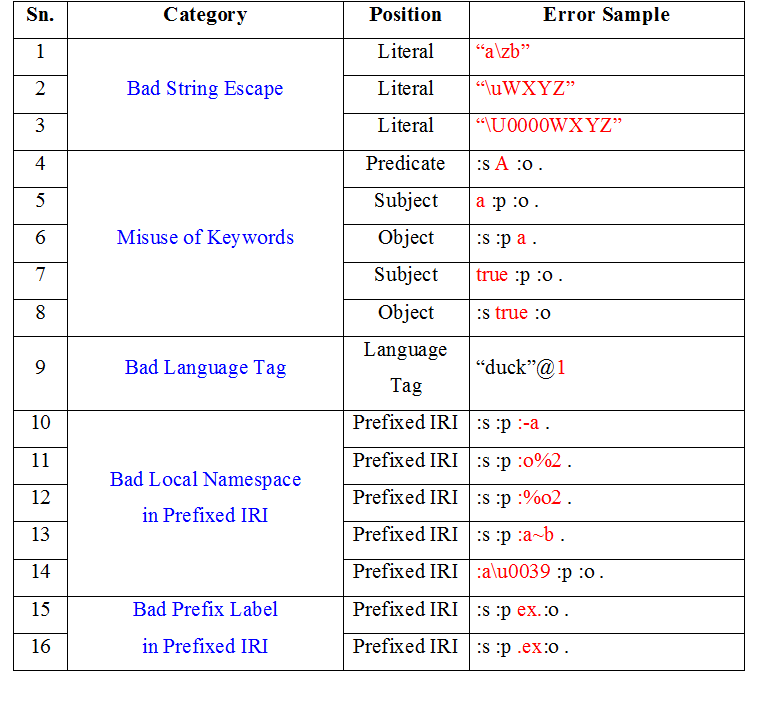
\includegraphics[width=5.5in]{images/bigTablePage1.png}
\end{table}

 \begin{figure}[H]
 	\centering
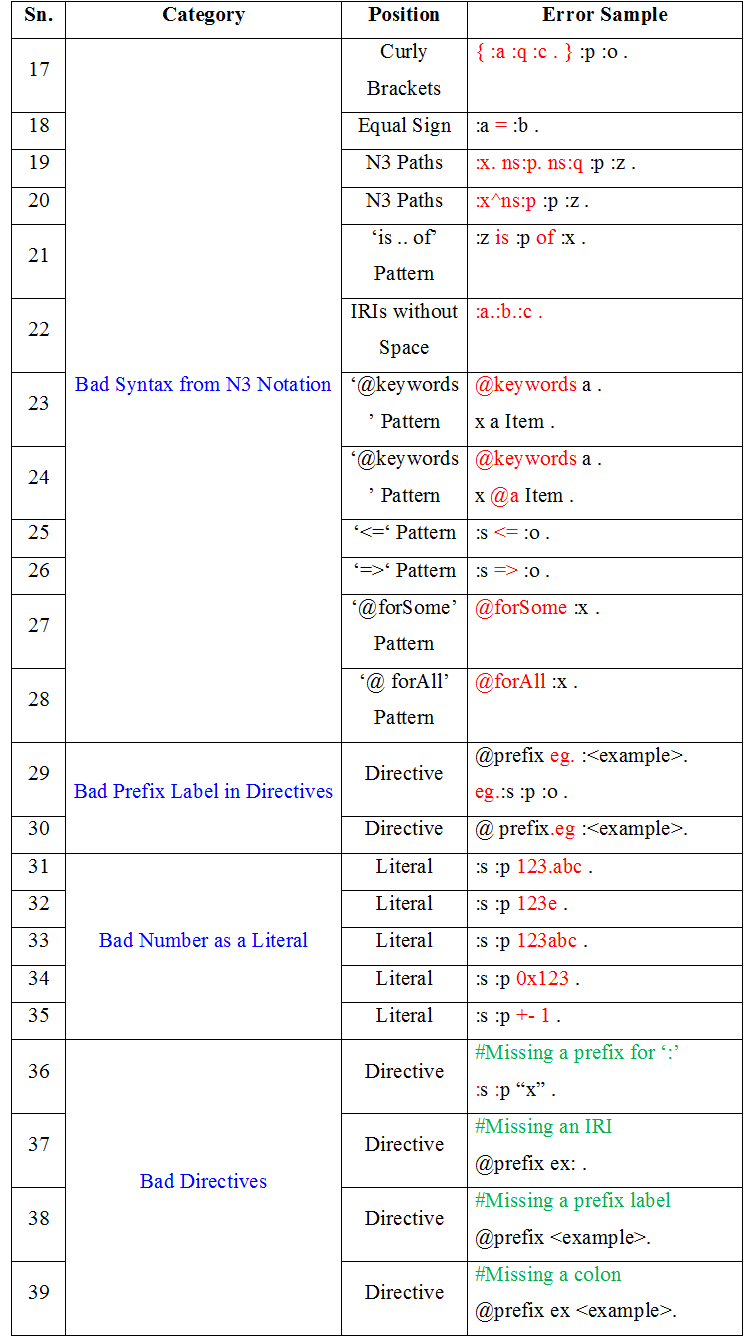
\includegraphics[width=5.5in]{images/bigTablePage3.png}
\end{figure}
 \begin{figure}[H]
 	\centering
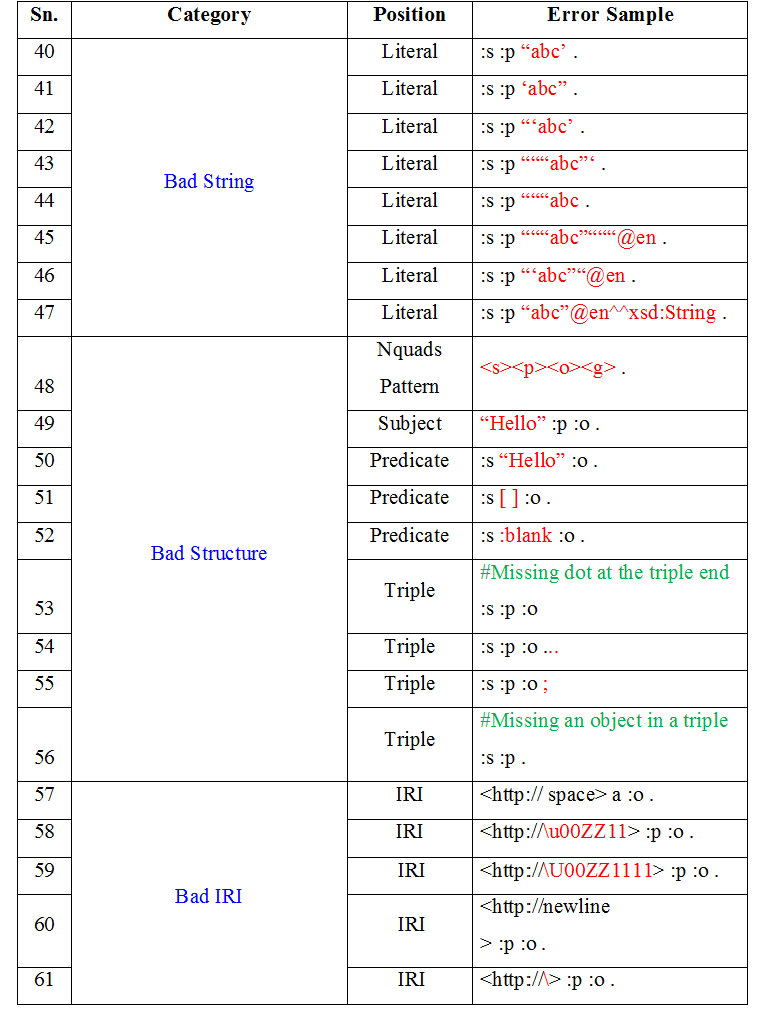
\includegraphics[width=5.5in]{images/bigTablePage7.png}
\end{figure}
%\includepdf[pages=2-3,pagecommand={},width=\textwidth,noautoscale=true,offset=80 30]{images/bigTable.pdf}
\end{appendices}


\end{document}  % The End
%% ----------------------------------------------------------------